\documentclass{beamer}


%%%%% 26-02-2022 package multicol multirow
\newcommand{\mc}[2]{\multicolumn{#1}{c}{#2}}
\definecolor{Gray}{gray}{0.85}
\definecolor{LightCyan}{rgb}{0.88,1,1}
\usepackage{hhline,longtable}
\usepackage{tabularx,booktabs}

\usepackage{multicol}
\usepackage{multirow}
%% 26-02-2022
\usepackage{hhline,longtable}
\usepackage{threeparttable}

\usepackage{tabularx,booktabs}
\newcommand{\tabitem}{~~\llap{\textbullet}~~}


\usepackage{enumerate}
\usepackage[shortlabels]{enumitem}

\setlist[enumerate, 1]{label =\textbf{\arabic*.}}
\setlist[enumerate, 2]{label =\textbf{\theenumi \alph*}}
\usepackage{array,multirow}

\usepackage{amsmath,mathtools}

\usepackage{amssymb}
\usepackage{amsthm}
\usepackage{mathtools}



\DeclarePairedDelimiter\abs{\lvert}{\rvert}%
\DeclarePairedDelimiter\norm{\lVert}{\rVert}%

% Swap the definition of \abs* and \norm*, so that \abs
% and \norm resizes the size of the brackets, and the 
% starred version does not.
\makeatletter
\let\oldabs\abs
\def\abs{\@ifstar{\oldabs}{\oldabs*}}










%%%% animation package 21-09-2021
\usepackage{animate}


%%%%%%%%%%%%%%%%%09-09-2021\\\ copied from Webinarinnovation page
% Here I would like to make a new command to change the transparency of a photo and put it as a background photo
\usepackage{tikz}



%%%%%%%%%%%% 22-10-2020 Background block package
% beamer: How to place images behind text (z-order)
% (http://tex.stackexchange.com/a/134311)
\makeatletter
\newbox\@backgroundblock
\newenvironment{backgroundblock}[2]{%
  \global\setbox\@backgroundblock=\vbox\bgroup%
    \unvbox\@backgroundblock%
    \vbox to0pt\bgroup\vskip#2\hbox to0pt\bgroup\hskip#1\relax%
}{\egroup\egroup\egroup}
\addtobeamertemplate{background}{\box\@backgroundblock}{}
\makeatother

%%%%%%%%%%%%%%%%%%%%%%%%%%%%%%%%%%%%%%%%%%%%
%%%%%%%%%%%26-10-2020% set figure number
\setbeamertemplate{caption}[numbered]


%%%%%%%%%%%%%%%%26-10-2020
\usepackage{amssymb,amsmath}


%%%%%%%%%%%%%%%%26-10-2020
\newenvironment{variableblock}[3]{%
  \setbeamercolor{block body}{#2}
  \setbeamercolor{block title}{#3}
  \begin{block}{#1}}{\end{block}}
  
  \setbeamercolor{block body alerted}{bg=alerted text.fg!10}
\setbeamercolor{block title alerted}{bg=alerted text.fg!20}
\setbeamercolor{block body}{bg=structure!10}
\setbeamercolor{block title}{bg=structure!20}
\setbeamercolor{block body example}{bg=green!10}
\setbeamercolor{block title example}{bg=green!20}

\setbeamertemplate{blocks}[rounded][shadow=true]


%%%%%%%%%%%%%%%%%%%%%26-10-2020
\setbeamertemplate{footline}[frame number]

%%%%%%%%%%%% 26-10-2020
\usepackage{color, colortbl}
\definecolor{Gray}{gray}{0.85}

%%%%%%%%%%%%%%%%%%27-10-2020
\usepackage[T1]{fontenc}



\title{\large \textbf{Large-Scale Integration of EVs, one Application of the High-Performace Solver: BATTPOWER}}
\begin{backgroundblock}{20mm}{20mm}
    \begin{tikzpicture}
    \node[anchor=east,inner sep=0] (B) at (4,0) {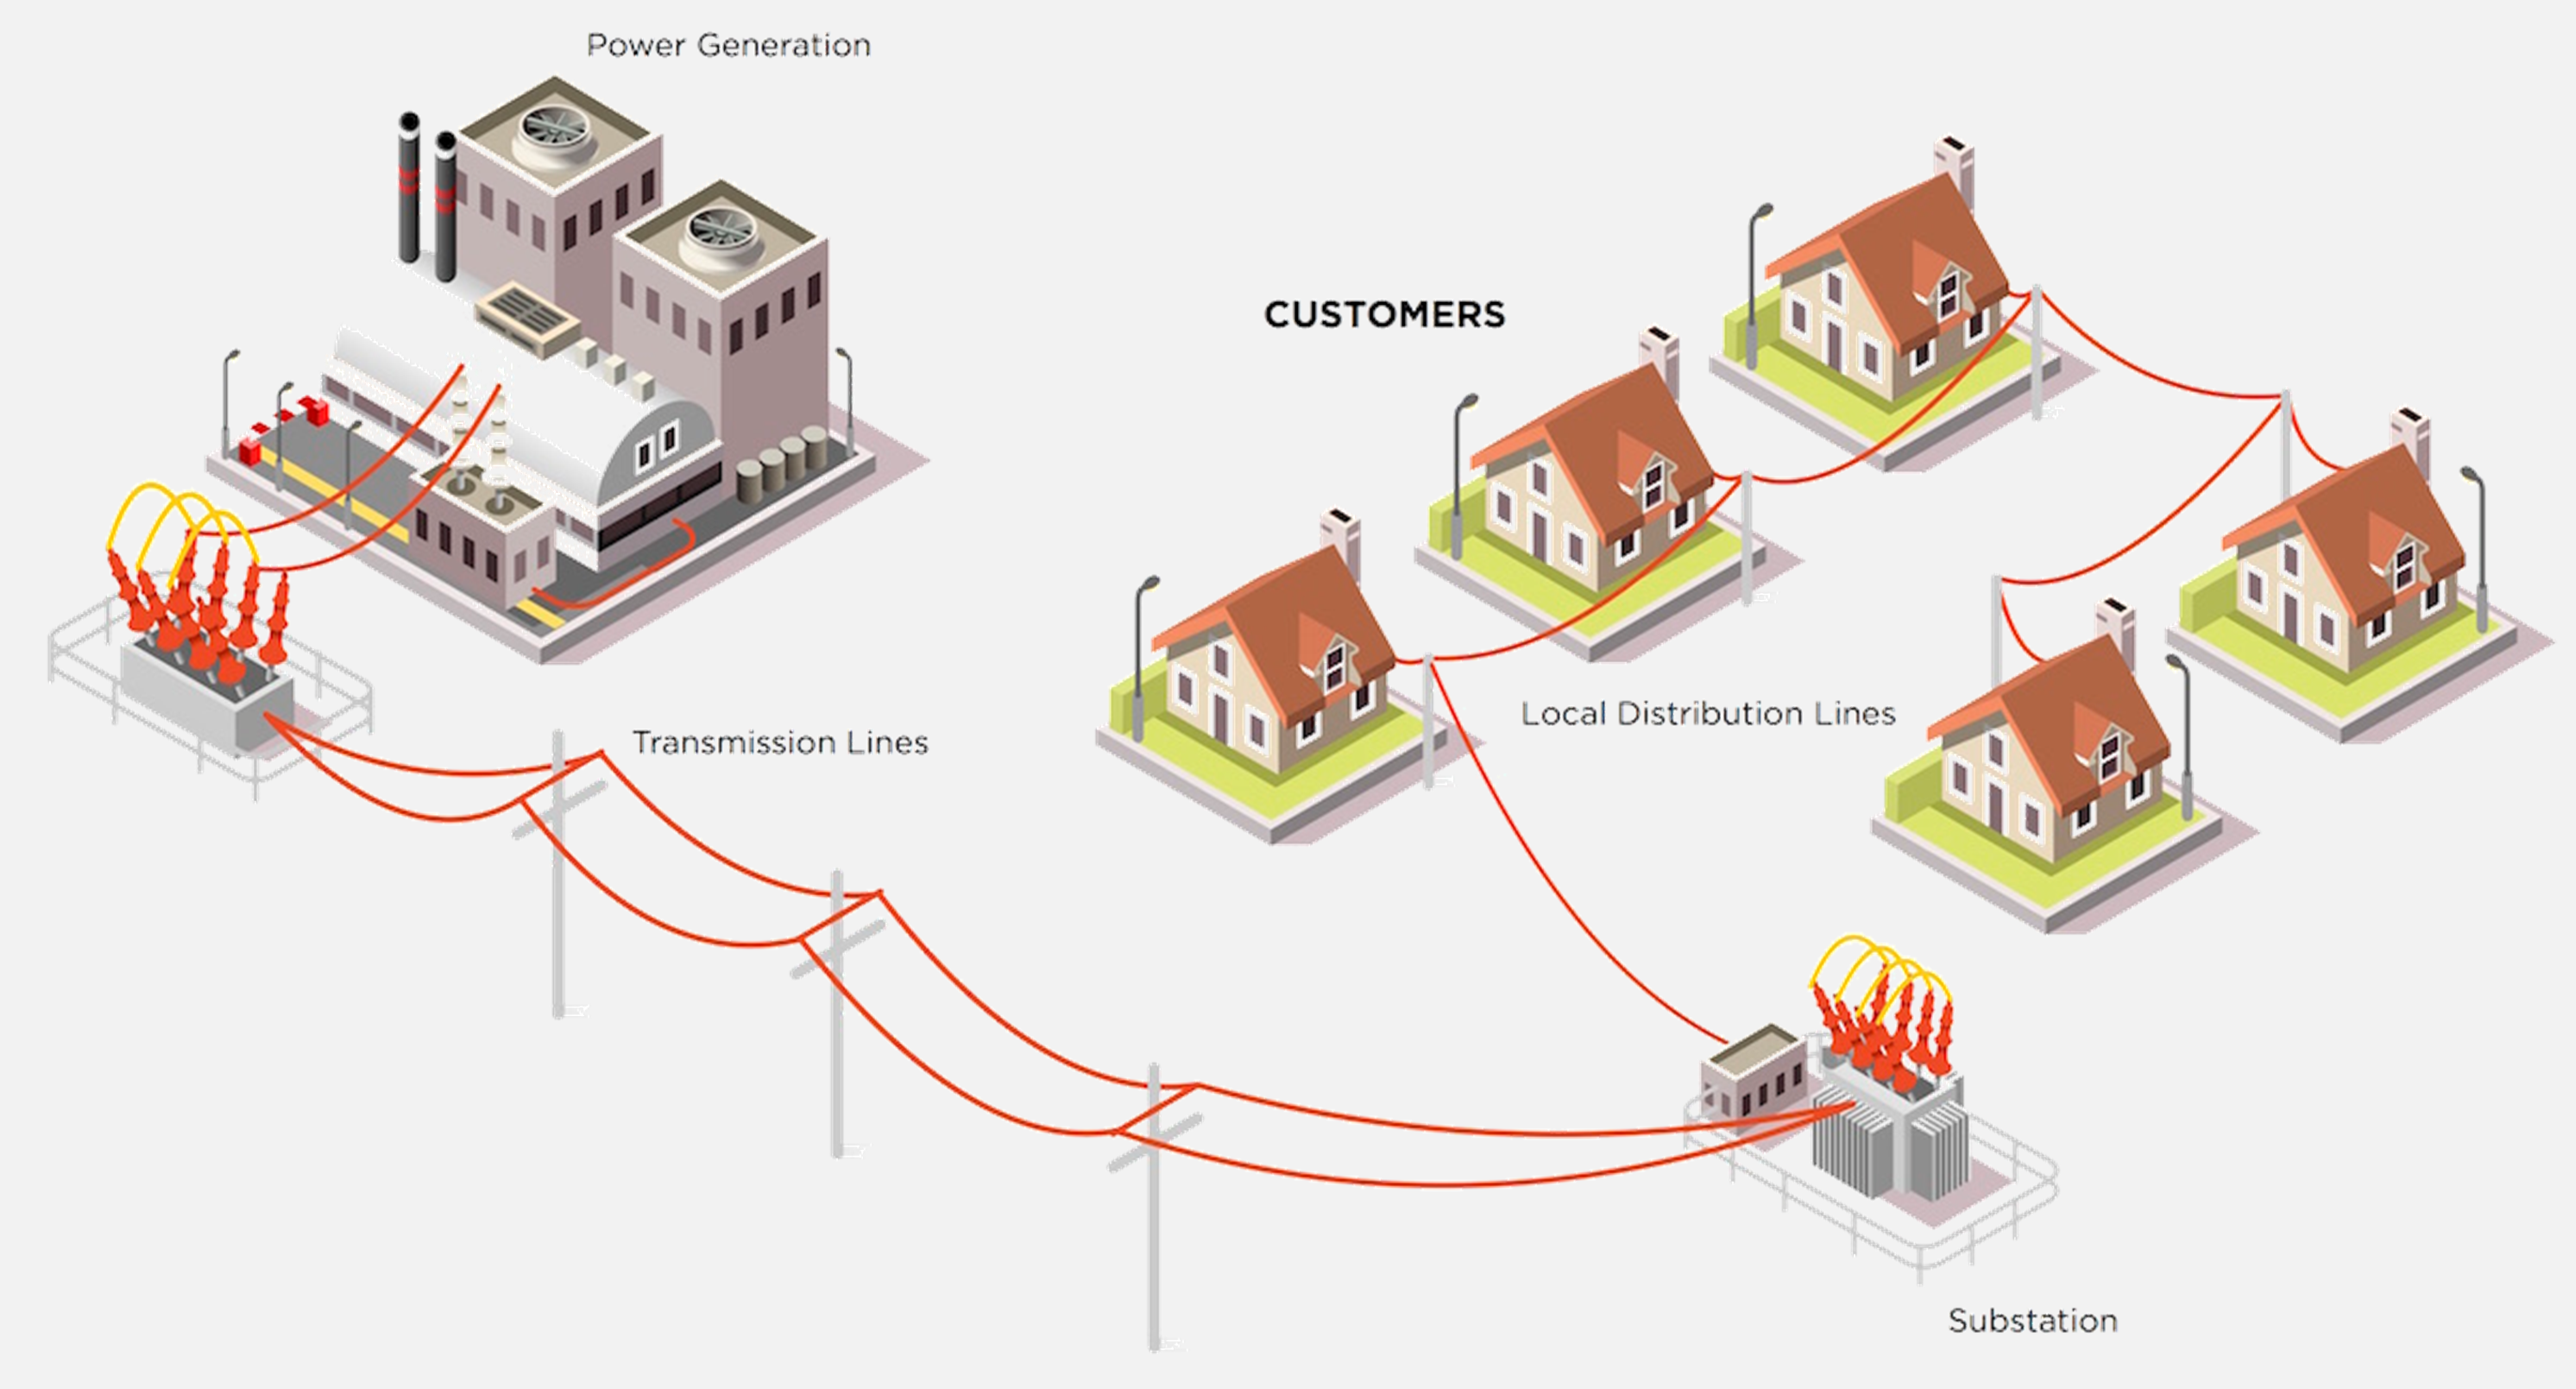
\includegraphics[width=\linewidth]{Figures/PowerSys.png}};
           \fill [draw=none, fill=white, fill opacity=0.7] (B.north west) -- (B.north east) -- (B.south east) -- (B.south west) -- (B.north west) -- cycle;
 
    \end{tikzpicture} 
    \end{backgroundblock} 

\logo{%
    
\includegraphics[width=3cm,height=3cm,keepaspectratio]{ntnulogo_eng}~%
}


\author{Salman Zaferanlouei}
\institute{NTNU{\\ \vskip 1cm} \scalebox{1.5}{\insertlogo}}
\date{\today}









\begin{document}
\begin{frame}
\titlepage
\end{frame}
%%%%%%%%%%%%%%%%%%%%%%%%%%%%%%%%%%%%%%%%%%
%%%%%%%%%%%%%%%%%%%%%%%%%%%%%%%%%%%%%%%%%%
%%%%%%%%%%%%%%%%%%%%%%%%%%%%%%%%%%%%%%%%%%
%%%%%%%%%%%%%%%%%%%%%%%%%%%%%%%%%%%%%%%%%%
\begin{frame}{Content}
\begin{itemize}
\item \textbf{Purpose:} Understanding of fast frequency reserve and current practice in Norway
\item \textbf{Time}: 45 min
\item \textbf{Target:} Public Audience
\item \textbf{How:} 
\end{itemize}
\begin{center}
\begin{tabular}{|l|} 
\hline
\rowcolor{Gray} \textbf{Inertia:} Physics of the power system \\
 \textbf{checkpoint I}\\
 \rowcolor{Gray} \textbf{TSO (Statnett):} Pilot Project 2018\\
 \textbf{checkpoint II}\\
 \rowcolor{Gray} \textbf{Concluding Remarks}\\
\hline
\end{tabular}
\end{center}



\end{frame}
%%%%%%%%%%%%%%%%%%%%%%%%%%%%%%%%%%%%%%%%%%
%%%%%%%%%%%%%%%%%%%%%%%%%%%%%%%%%%%%%%%%%%
%%%%%%%%%%%%%%%%%%%%%%%%%%%%%%%%%%%%%%%%%%
%%%%%%%%%%%%%%%%%%%%%%%%%%%%%%%%%%%%%
\section{Introduction to Power System Inertia}
\begin{frame}{The Electricity System}
\begin{block}{Characteristics of power system}
\begin{itemize}
\item power system with suppliers and consumers
\item power generated cannot be stored largely, so it must be consumed
\item the entire system is in a frequency balance of 50 Hz and needs to be maintained 
\end{itemize}
\end{block}
\begin{figure}
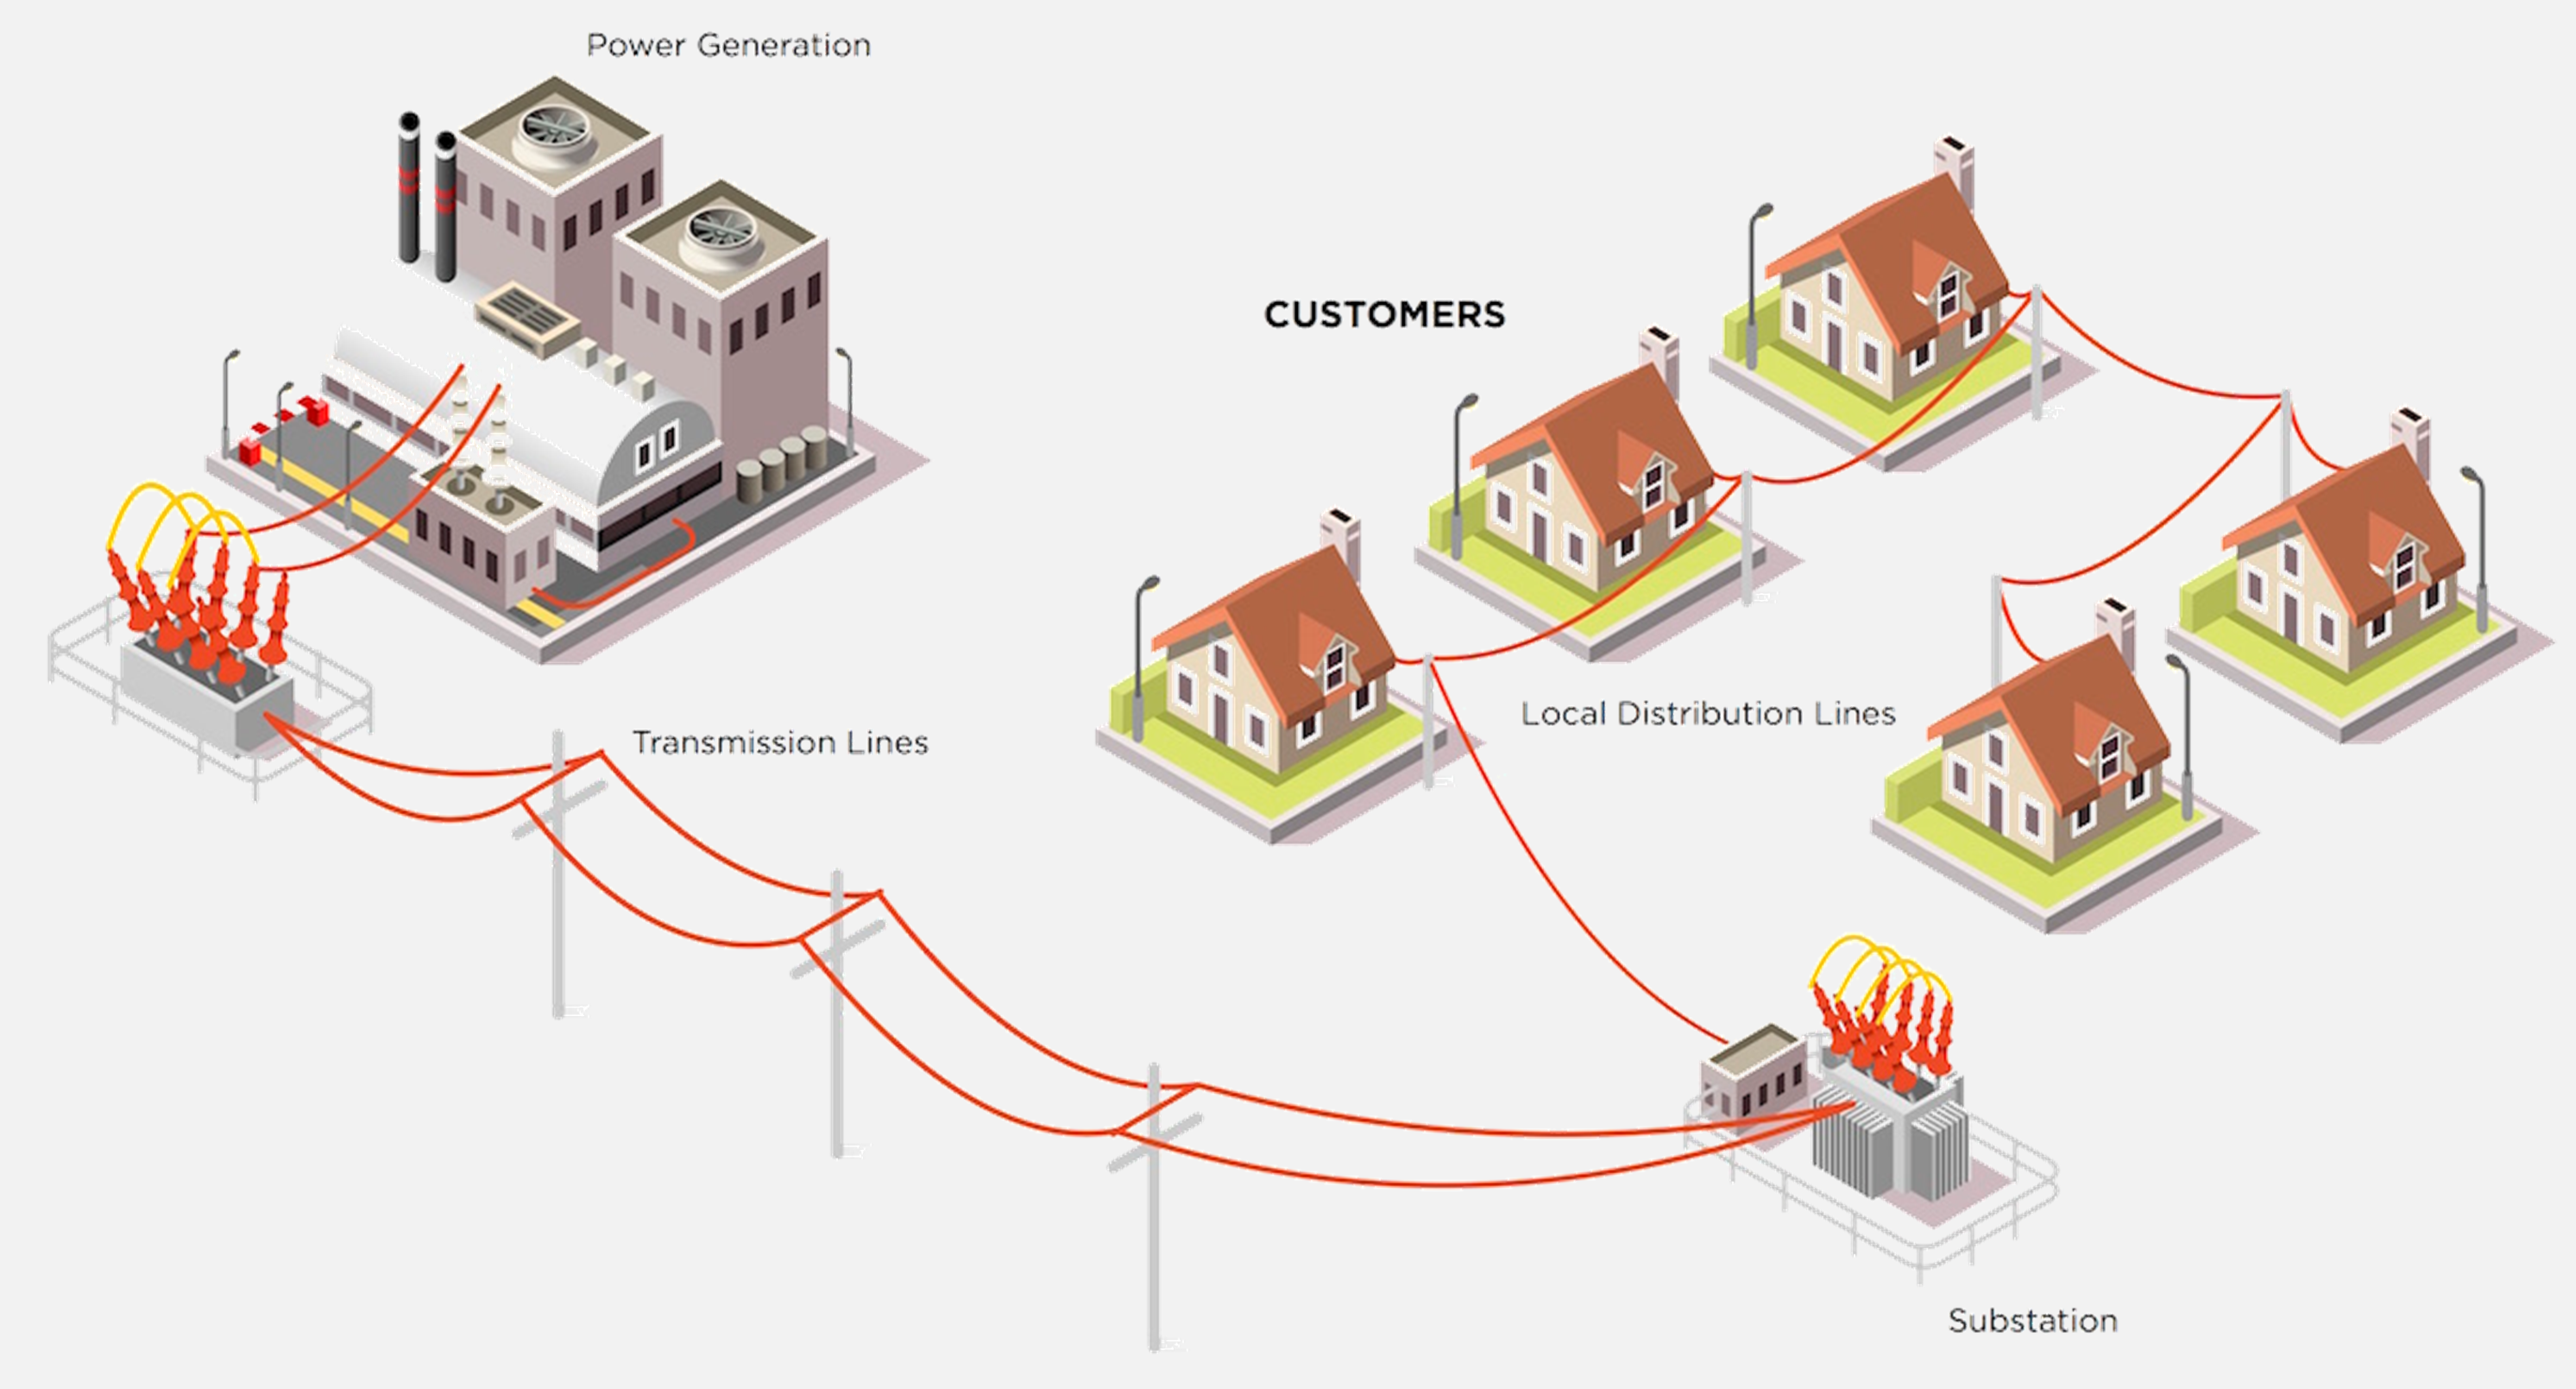
\includegraphics[scale=0.1]{Figures/PowerSys.png}
 \caption{A Typical Power System \textcolor{gray}{\tiny[Rochester Gas \& Electricity]}}
\end{figure}

\end{frame}
%%%%%%%%%%%%%%%%%%%%%%%%%%%%%%%%%%%%%%%%%%
%%%%%%%%%%%%%%%%%%%%%%%%%%%%%%%%%%%%%%%%%%
%%%%%%%%%%%%%%%%%%%%%%%%%%%%%%%%%%%%%%%%%%
%%%%%%%%%%%%%%%%%%%%%%%%%%%%%%%%%%%%%%%%%%
\section{Frequency and Oscillation}
\subsection{steady-state}
\begin{frame}{Steady-State: Balance Model}
\begin{block}{Supply = Demand}
Simplest model of a power system can be written as a balance model 
\end{block}
        \begin{figure}
        \includegraphics[scale=0.35]{Figures/steadystate.PNG}
        \caption{Steady-state balance model of power systems  \textcolor{gray}{\tiny [figure adapted from “Power system dynamics visualization . . . ” by F. Milano ’18]}}
        \end{figure}

\end{frame}

%%%%%%%%%%%%%%%%%%%%%%%%%%%%%%%%%%%%%%%%%%
%%%%%%%%%%%%%%%%%%%%%%%%%%%%%%%%%%%%%%%%%%
%%%%%%%%%%%%%%%%%%%%%%%%%%%%%%%%%%%%%%%%%%
%%%%%%%%%%%%%%%%%%%%%%%%%%%%%%%%%%%%%%%%%%
\subsection{Dynamic}
\begin{frame}
\begin{block}{Inertia and Electromechanical Oscillations}
Let us assume for now that the system includes synchronous machines but no control.\\
\centering  $Ma-F=0$\\
\centering $M\ddot{\theta}-K\theta=0$\\
\centering $M\ddot{\theta}-[P_{gen}-P_{load}]=0$
\end{block}
        \begin{figure}
        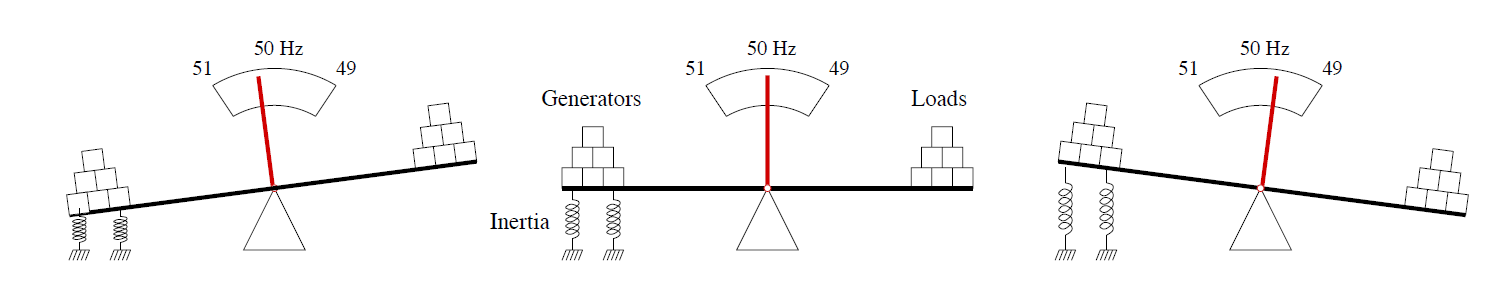
\includegraphics[scale=0.35]{Figures/SystemInertia1.PNG}
        \caption{Mechanical springs represent the synchronous machine inertia \textcolor{gray}{\tiny [figure adapted from “Power system dynamics visualization . . . ” by F. Milano ’18]}}
        \end{figure}

\end{frame}


%%%%%%%%%%%%%%%%%%%%%%%%%%%%%%%%%%%%%%%%%%
%%%%%%%%%%%%%%%%%%%%%%%%%%%%%%%%%%%%%%%%%%
%%%%%%%%%%%%%%%%%%%%%%%%%%%%%%%%%%%%%%%%%%
%%%%%%%%%%%%%%%%%%%%%%%%%%%%%%%%%%%%%%%%%%
\subsection{Frequency Control}
\begin{frame}{Primary Frequency Control}
\begin{block}{Notation}
{\tiny To represent the primary frequency control, we connect a mass to the fulcrum of the beam to lower
the center of mass of the scale. Moreover, we add mechanical dampers. Whenever an unbalanced condition occurs, the scale will start to oscillate
but the effect of the damper will prevent a sustained oscillation around the equilibrium point. Then the
new equilibrium is given by the sum of the momenta of the three masses, generators, loads and
primary frequency control.}
\end{block}

        \begin{figure}
        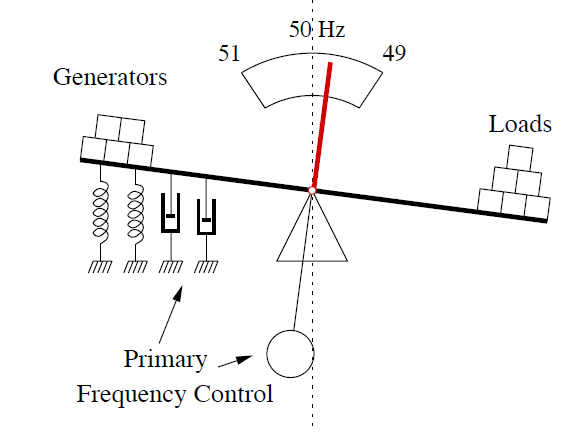
\includegraphics[scale=0.35]{Figures/SystemInertia.PNG}
        \caption{\textcolor{gray}{\tiny [figure adapted from “Power system dynamics visualization . . . ” by F. Milano ’18]}}
        \end{figure}

\end{frame}

%%%%%%%%%%%%%%%%%%%%%%%%%%%%%%%%%%%%%%%%%%
%%%%%%%%%%%%%%%%%%%%%%%%%%%%%%%%%%%%%%%%%%
%%%%%%%%%%%%%%%%%%%%%%%%%%%%%%%%%%%%%%%%%%
%%%%%%%%%%%%%%%%%%%%%%%%%%%%%%%%%%%%%%%%%%
\begin{frame}{Secondary Frequency Control}
\begin{block}{Notation}
{\tiny This is basically just a
rescheduling of the active power set point of the turbines of the synchronous machines. The AGC is
much slower than the primary frequency control and in the mechanical model its effect
is mainly visible at the equilibrium. The representation in the figure is simplistic, however. In practice all generators will increase their power production to compensate a generator outage or a load
increase.}
\end{block}

        \begin{figure}
        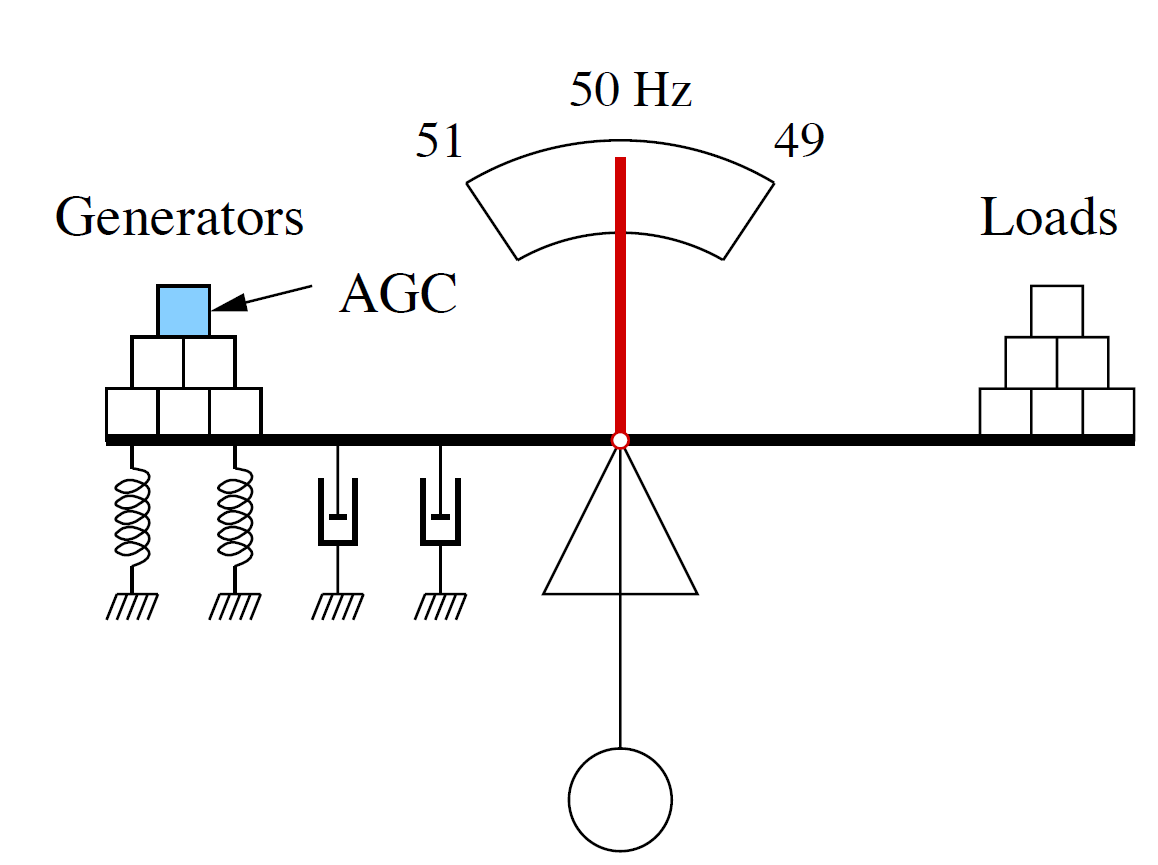
\includegraphics[scale=0.2]{Figures/SystemInertia3.PNG}
        \caption{\textcolor{gray}{\tiny [figure adapted from “Power system dynamics visualization . . . ” by F. Milano ’18]}}
        \end{figure}

\end{frame}
%%%%%%%%%%%%%%%%%%%%%%%%%%%%%%%%%%%%%%%%%%
%%%%%%%%%%%%%%%%%%%%%%%%%%%%%%%%%%%%%%%%%%
%%%%%%%%%%%%%%%%%%%%%%%%%%%%%%%%%%%%%%%%%%
%%%%%%%%%%%%%%%%%%%%%%%%%%%%%%%%%%%%%%%%%%
\begin{frame}{Effect of renewable generations}
\begin{block}{Notation}
{\tiny Renewable sources have several effects on the system: they add randomness and reduce
inertia, spinning reserve and damping.}
\end{block}

        \begin{figure}
        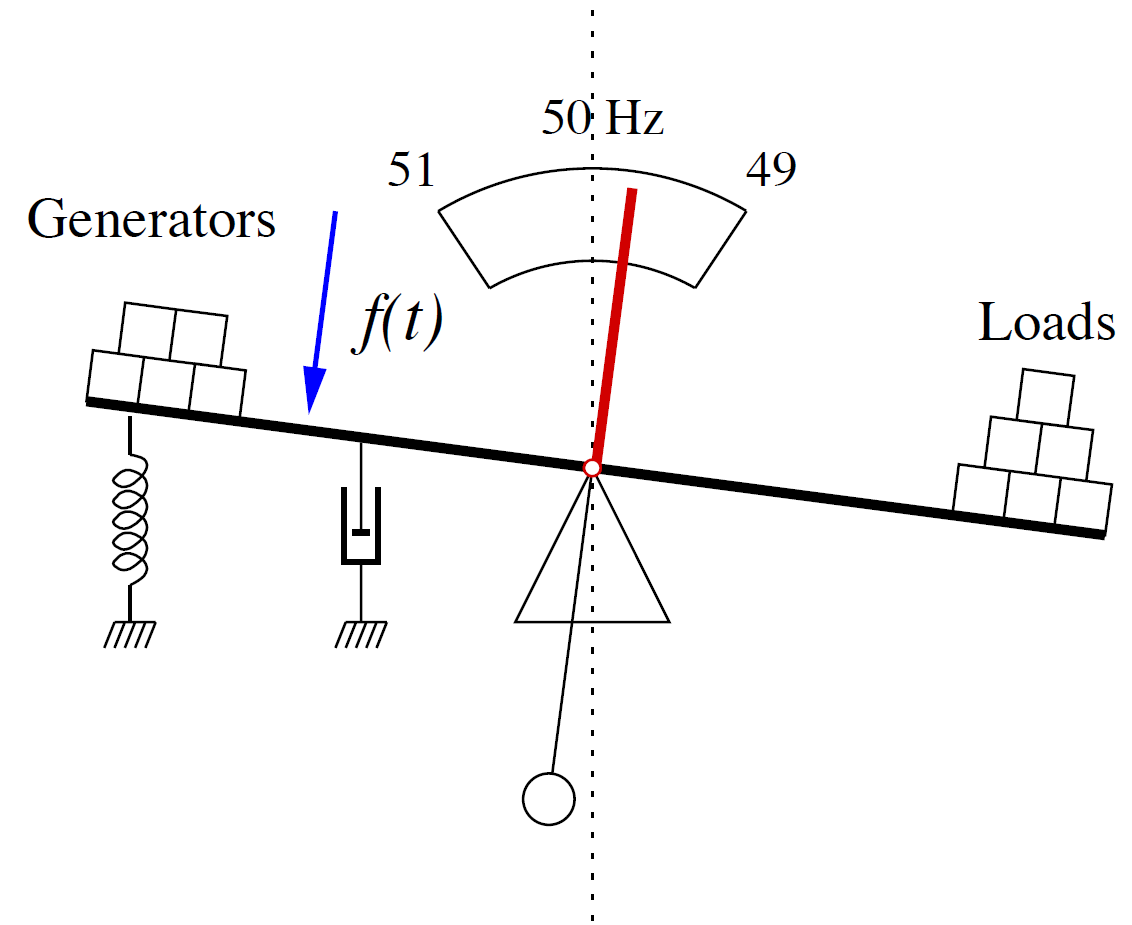
\includegraphics[scale=0.2]{Figures/SystemInertia4.PNG}
        \caption{\textcolor{gray}{\tiny [figure adapted from “Power system dynamics visualization . . . ” by F. Milano ’18]}}
        \end{figure}

\end{frame}

%%%%%%%%%%%%%%%%%%%%%%%%%%%%%%%%%%%%%%%%%%
%%%%%%%%%%%%%%%%%%%%%%%%%%%%%%%%%%%%%%%%%%
%%%%%%%%%%%%%%%%%%%%%%%%%%%%%%%%%%%%%%%%%%
%%%%%%%%%%%%%%%%%%%%%%%%%%%%%%%%%%%%%%%%%%
\begin{frame}{Effect of renewable generations}
\begin{block}{Notation}
{\centering $\textcolor{red}{M \ddot{\theta}}=P_{generation}(t)-P_{demand}(t) $\\
change of kinetic energy = instantaneous power balance}
\end{block}

 


 \begin{columns}
    \column{0.6\textwidth}
    \begin{figure}
        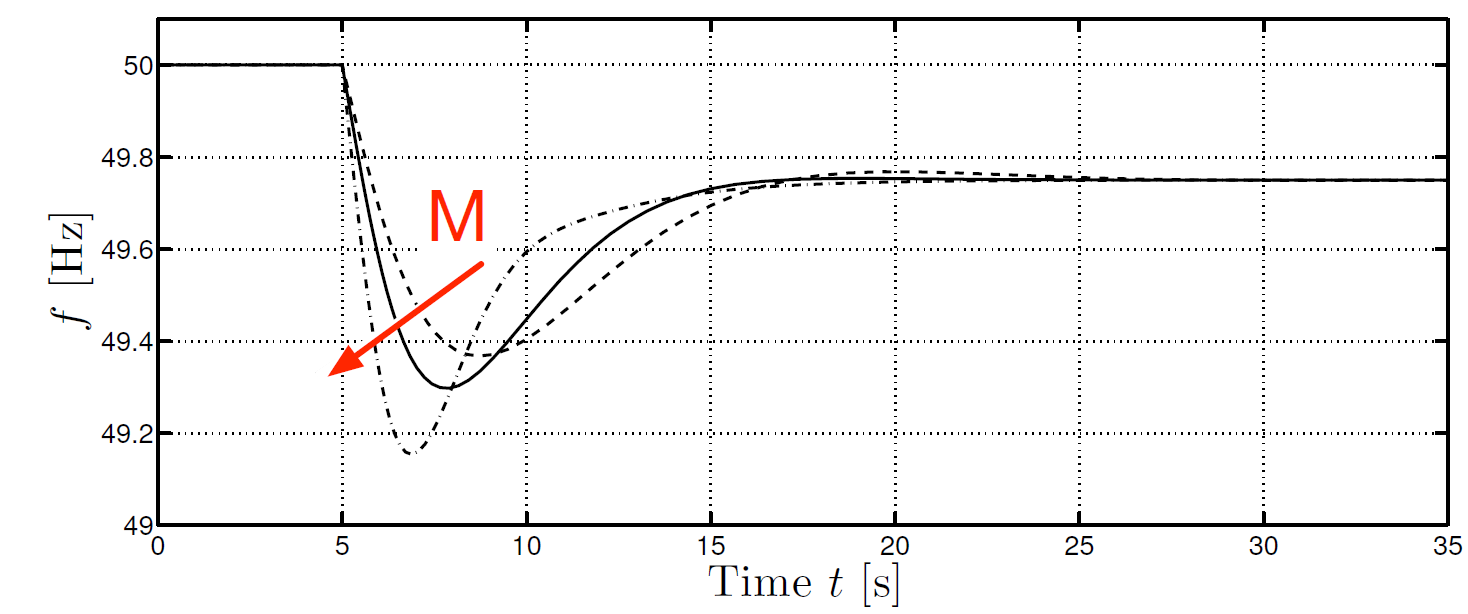
\includegraphics[scale=0.2]{Figures/SystemInertia5.PNG}
        \caption{\textcolor{gray}{\tiny [figure adapted from “Low-Inertia Power Systems . . . ” by Florian Dörfler, ETH Zurich]}}
        \end{figure}
    \column{0.4\textwidth}
        \begin{figure}
        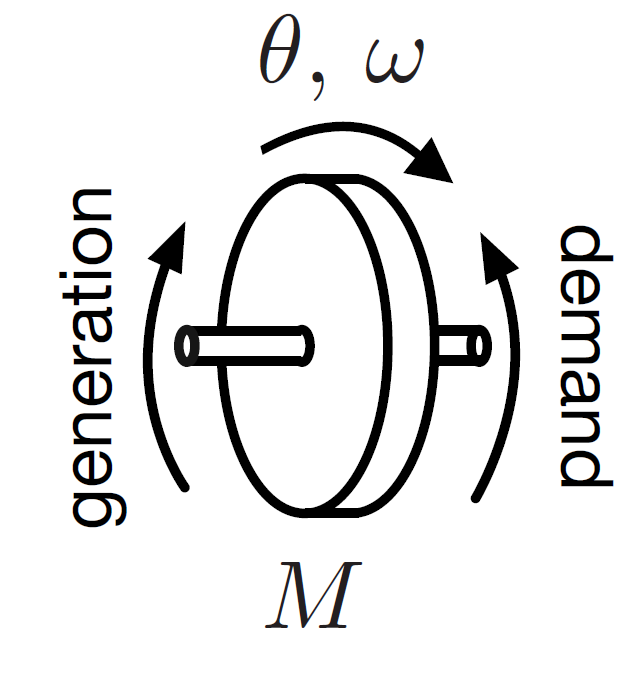
\includegraphics[scale=0.2]{Figures/SystemInertia6.PNG}
\caption{\textcolor{gray}{\tiny [figure adapted from “Low-Inertia Power Systems . . . ” by Florian Dörfler, ETH Zurich]}}
        \end{figure}
\end{columns}



\end{frame}
%%%%%%%%%%%%%%%%%%%%%%%%%%%%%%%%%%%%%%%%%%
%%%%%%%%%%%%%%%%%%%%%%%%%%%%%%%%%%%%%%%%%%
%%%%%%%%%%%%%%%%%%%%%%%%%%%%%%%%%%%%%%%%%%
%%%%%%%%%%%%%%%%%%%%%%%%%%%%%%%%%%%%%%%%%%
\begin{frame}
\begin{block}{RoCoF}
Rate of Change of Frequency = RoCoF\\
\end{block}
\begin{itemize}
\item<1-> M $\textcolor{red}{\uparrow}$ \quad RoCoF $\textcolor{red}{\downarrow}$
\item<2-> M $\textcolor{red}{\downarrow}$ \quad RoCoF $\textcolor{red}{\uparrow}$
\end{itemize}
\begin{figure}
\includegraphics[scale=0.3]{Figures/RoCoF.PNG}
\caption{\textcolor{gray}{\tiny [figure adapted from “Fast Frequency Reserve – Solution to the Nordic inertia challenge ” by entsoe]}}
\end{figure}
\end{frame}

%%%%%%%%%%%%%%%%%%%%%%%%%%%%%%%%%%%%%%%%%%
%%%%%%%%%%%%%%%%%%%%%%%%%%%%%%%%%%%%%%%%%%
%%%%%%%%%%%%%%%%%%%%%%%%%%%%%%%%%%%%%%%%%%
%%%%%%%%%%%%%%%%%%%%%%%%%%%%%%%%%%%%%%%%%%
\section{Introduction to FFR}
\begin{frame}{Inertia in Power Systems}
\begin{itemize}
\item<1-> It is expected that electricity will be produced more and more by wind and solar power plants.
\only<1> {\begin{figure}
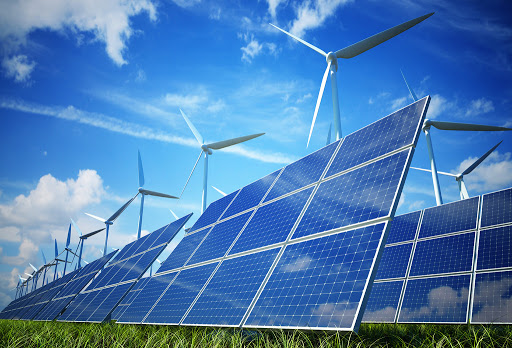
\includegraphics[width=50mm]{Figures/WindSolar.jpg}
 \caption{Wind and Solar \textcolor{gray}{\tiny [Source: Getty Images]}}
\end{figure}}

\addtocounter{figure}{1}

\item<2-> Thermal power plants will spend less time synchronised to the power system.
\only<2> {\begin{figure}
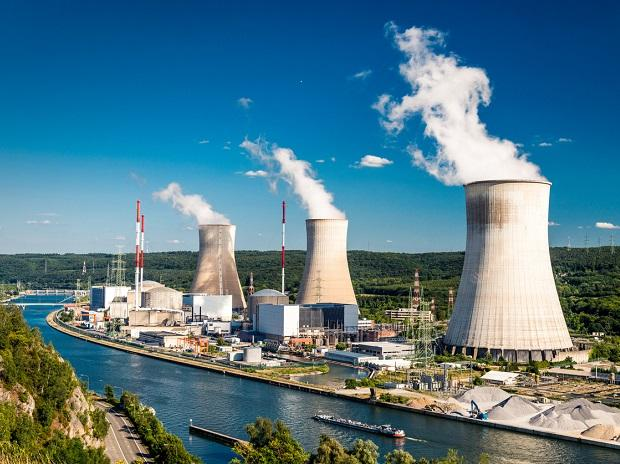
\includegraphics[width=50mm]{Figures/ThermalPowerPlant.jpg}
\caption{Thermal Power Plant \textcolor{gray}{\tiny[business-standard.com]}}
\end{figure}}



\item<3-> Consumption patterns due to electrification and smart control systems: Load characteristics are expected to continue to change, with rotating motors being connected to the power system through frequency converters.
\item<4-> High import on HVDC connections to other synchronous systems is also expected to replace traditional production more often.
\addtocounter{figure}{1}

\only<4> {\begin{figure}
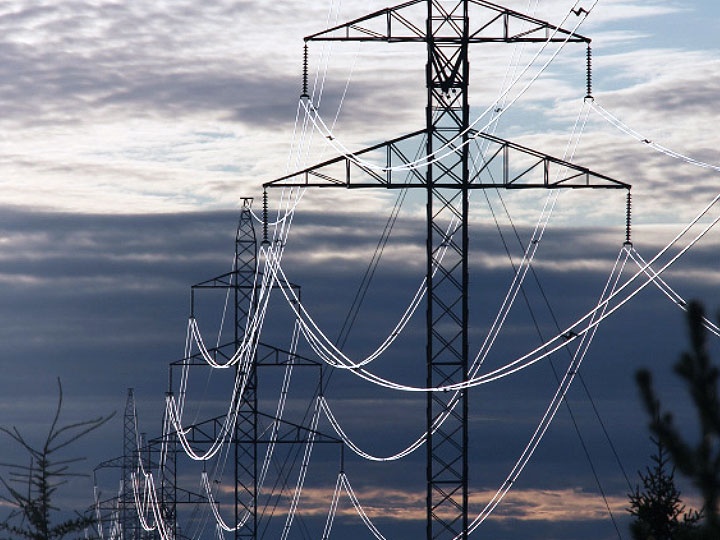
\includegraphics[width=30mm]{Figures/HVDC.jpg}
\caption{HVDC \textcolor{gray}{\tiny [etap.com]}}
\end{figure}}
\item<5-> Decommissioning of nuclear power plants.






\end{itemize}
\end{frame}
%%%%%%%%%%%%%%%%%%%%%%%%%%%%%%%%%%%%%%%%%%
%%%%%%%%%%%%%%%%%%%%%%%%%%%%%%%%%%%%%%%%%%
%%%%%%%%%%%%%%%%%%%%%%%%%%%%%%%%%%%%%%%%%%
%%%%%%%%%%%%%%%%%%%%%%%%%%%%%%%%%%%%%%%%%%
\section{Checkpoint II}
\begin{frame}{Checkpoint I}
\centering \begin{block}{}
\textbf{TSO (Statnett):} Pilot Project 2018
\end{block} 
\end{frame}
%%%%%%%%%%%%%%%%%%%%%%%%%%%%%%%%%%%%%%%%%%
%%%%%%%%%%%%%%%%%%%%%%%%%%%%%%%%%%%%%%%%%%
%%%%%%%%%%%%%%%%%%%%%%%%%%%%%%%%%%%%%%%%%%
%%%%%%%%%%%%%%%%%%%%%%%%%%%%%%%%%%%%%%%%%%
\begin{frame}{System Structure: Market and System Operators}
\addtocounter{figure}{1}

\begin{figure}
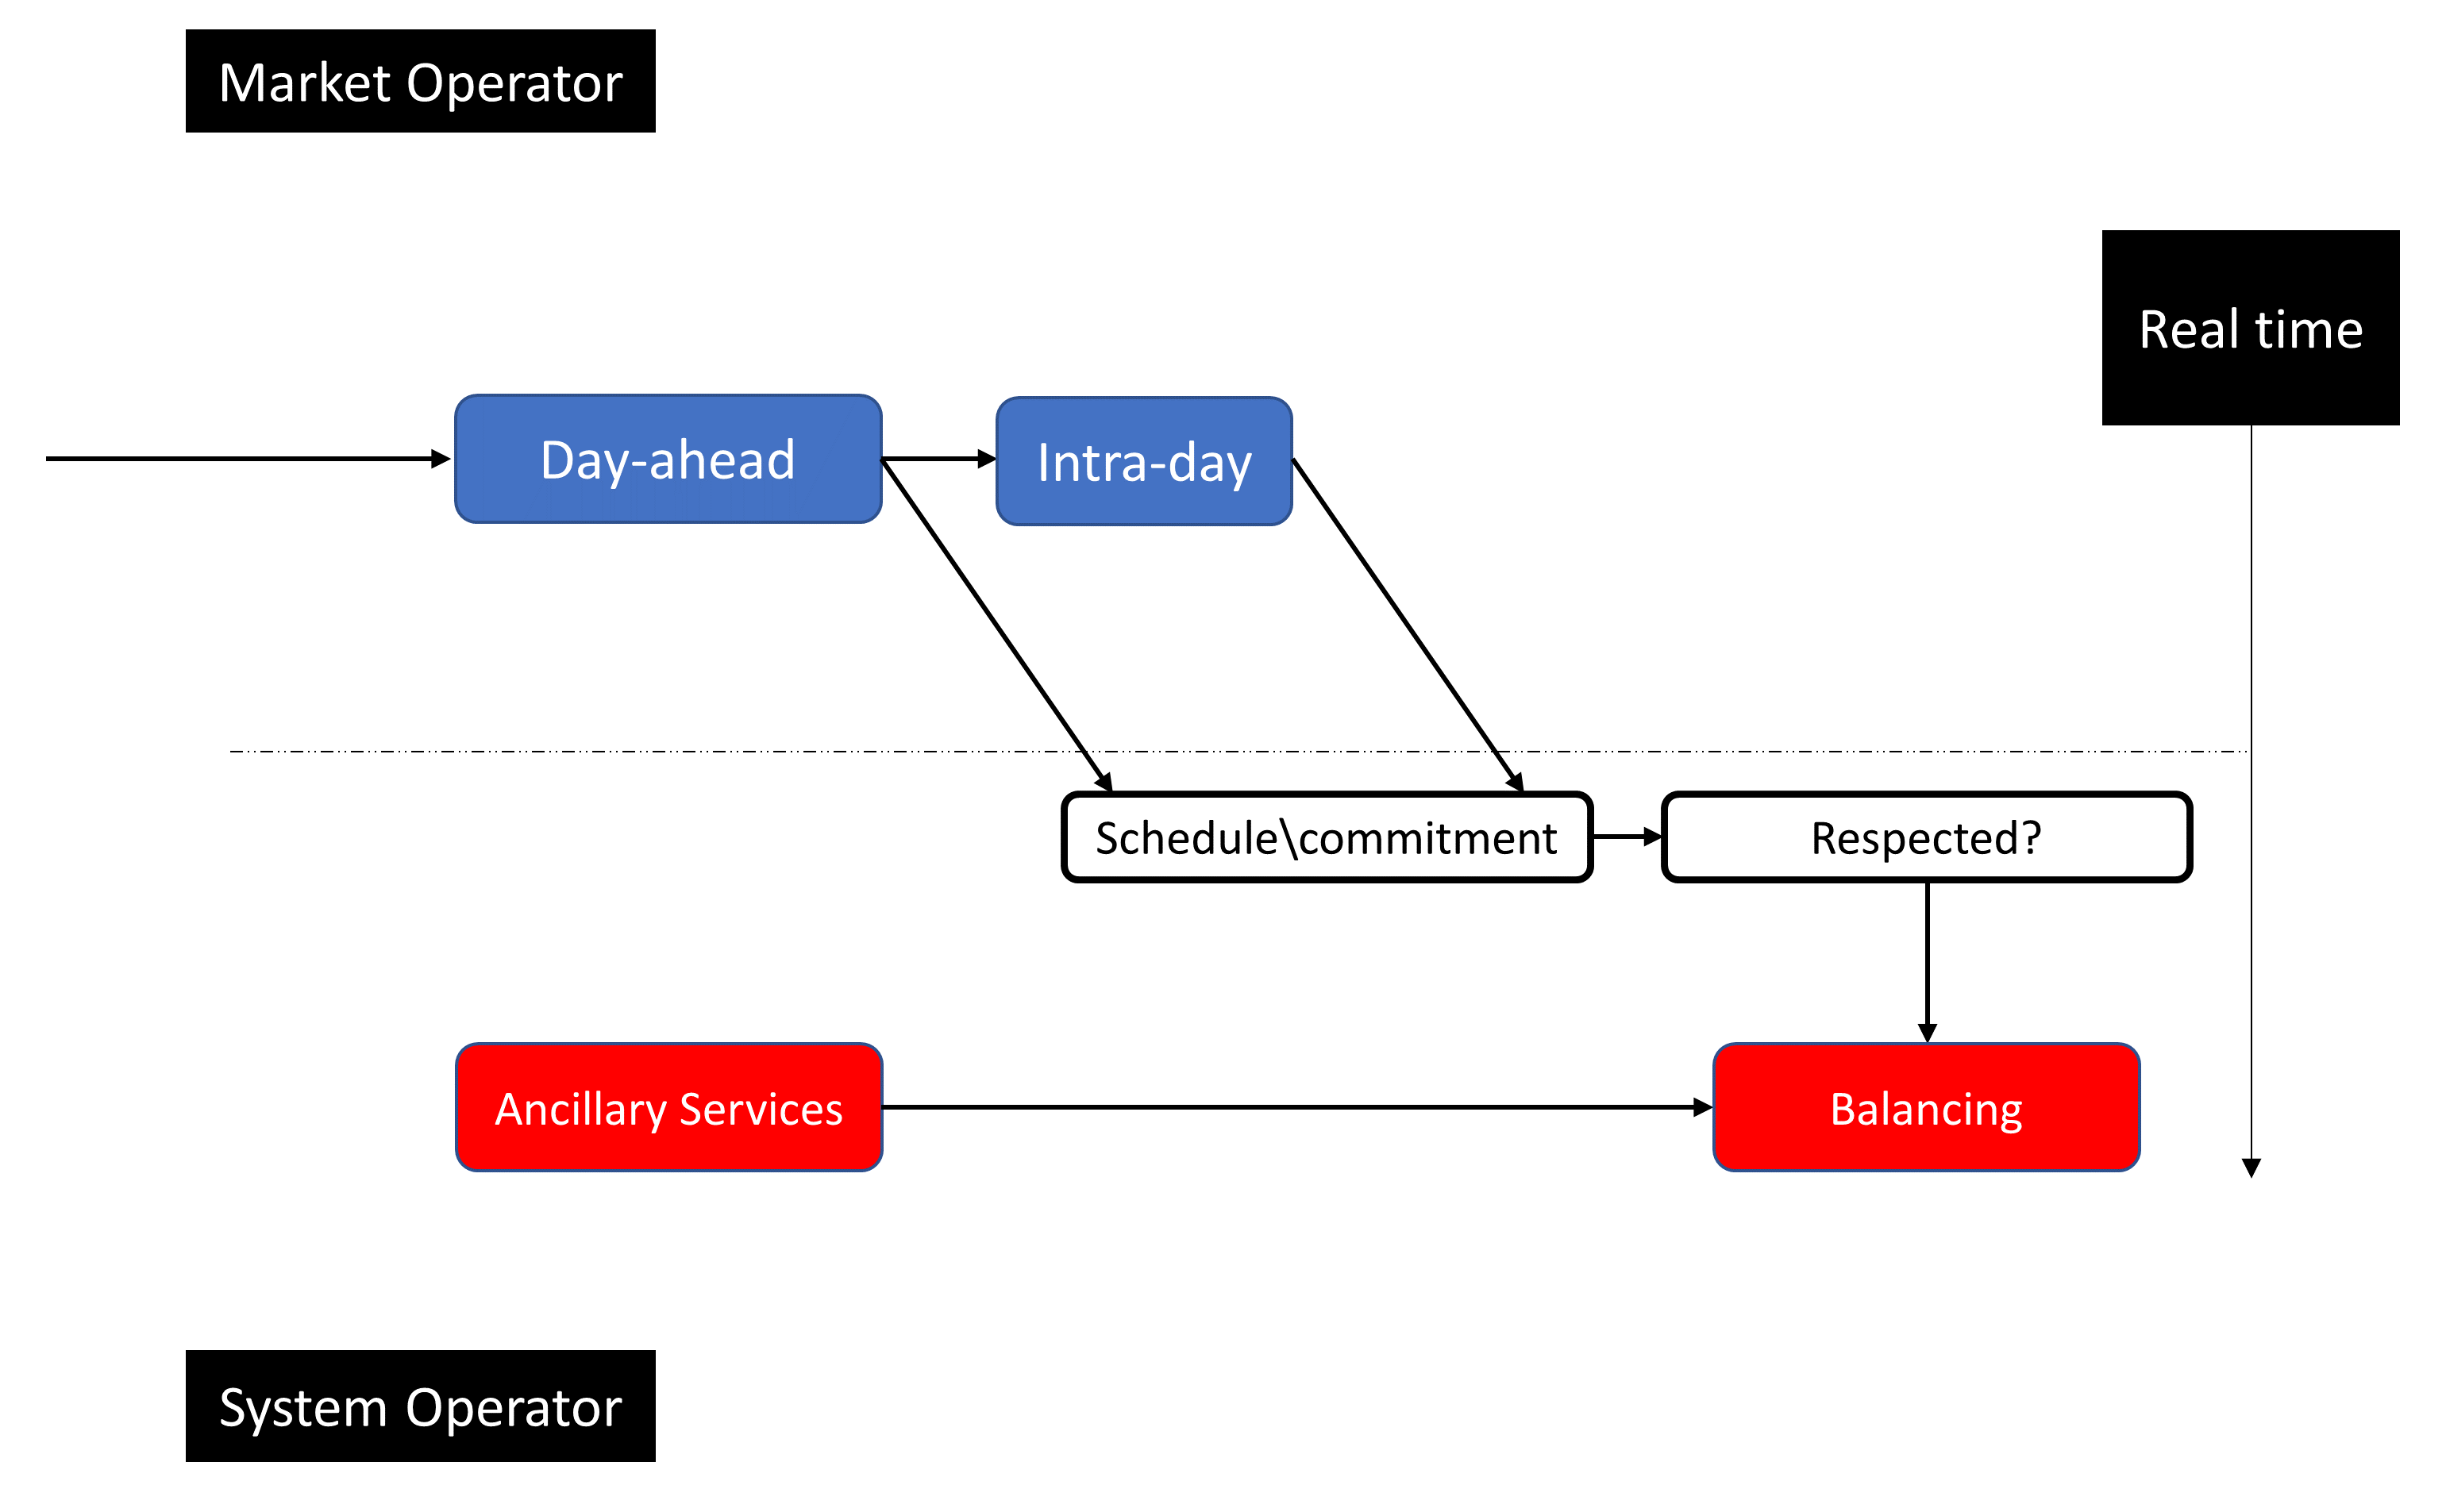
\includegraphics[width=90mm]{Figures/MarketModel.png}
\caption{Structure of Market and System Operator} 
\end{figure}

\end{frame}

%%%%%%%%%%%%%%%%%%%%%%%%%%%%%%%%%%%%%%%%%%
%%%%%%%%%%%%%%%%%%%%%%%%%%%%%%%%%%%%%%%%%%
%%%%%%%%%%%%%%%%%%%%%%%%%%%%%%%%%%%%%%%%%%
%%%%%%%%%%%%%%%%%%%%%%%%%%%%%%%%%%%%%%%%%%
\begin{frame}{The role of TSO-Operational Security}
\vskip -0.4cm
\begin{block}{Statnett duties:}
{\tiny
\begin{enumerate}
\item<1-> Balance production and consumption.
\item<2-> Maintain voltages throughout the power system.
\item<3-> Control power flows and avoid congestion.
\item<4-> Maintain the rotor angle stability to make sure there is no oscillations.
 
\item<5->    \hspace*{.1\linewidth}\begin{minipage}{.8\linewidth}
\begin{alertblock}{}
\textcolor{red}{Restore the system after blackout}
\end{alertblock} 
    \end{minipage}
   
\item<6-> Adapt the control system over time.
\end{enumerate}
}
\end{block}
\only<6> { \begin{alertblock}{}
Power system is more than 100 years old and changing a lot
\end{alertblock}
\begin{center}

 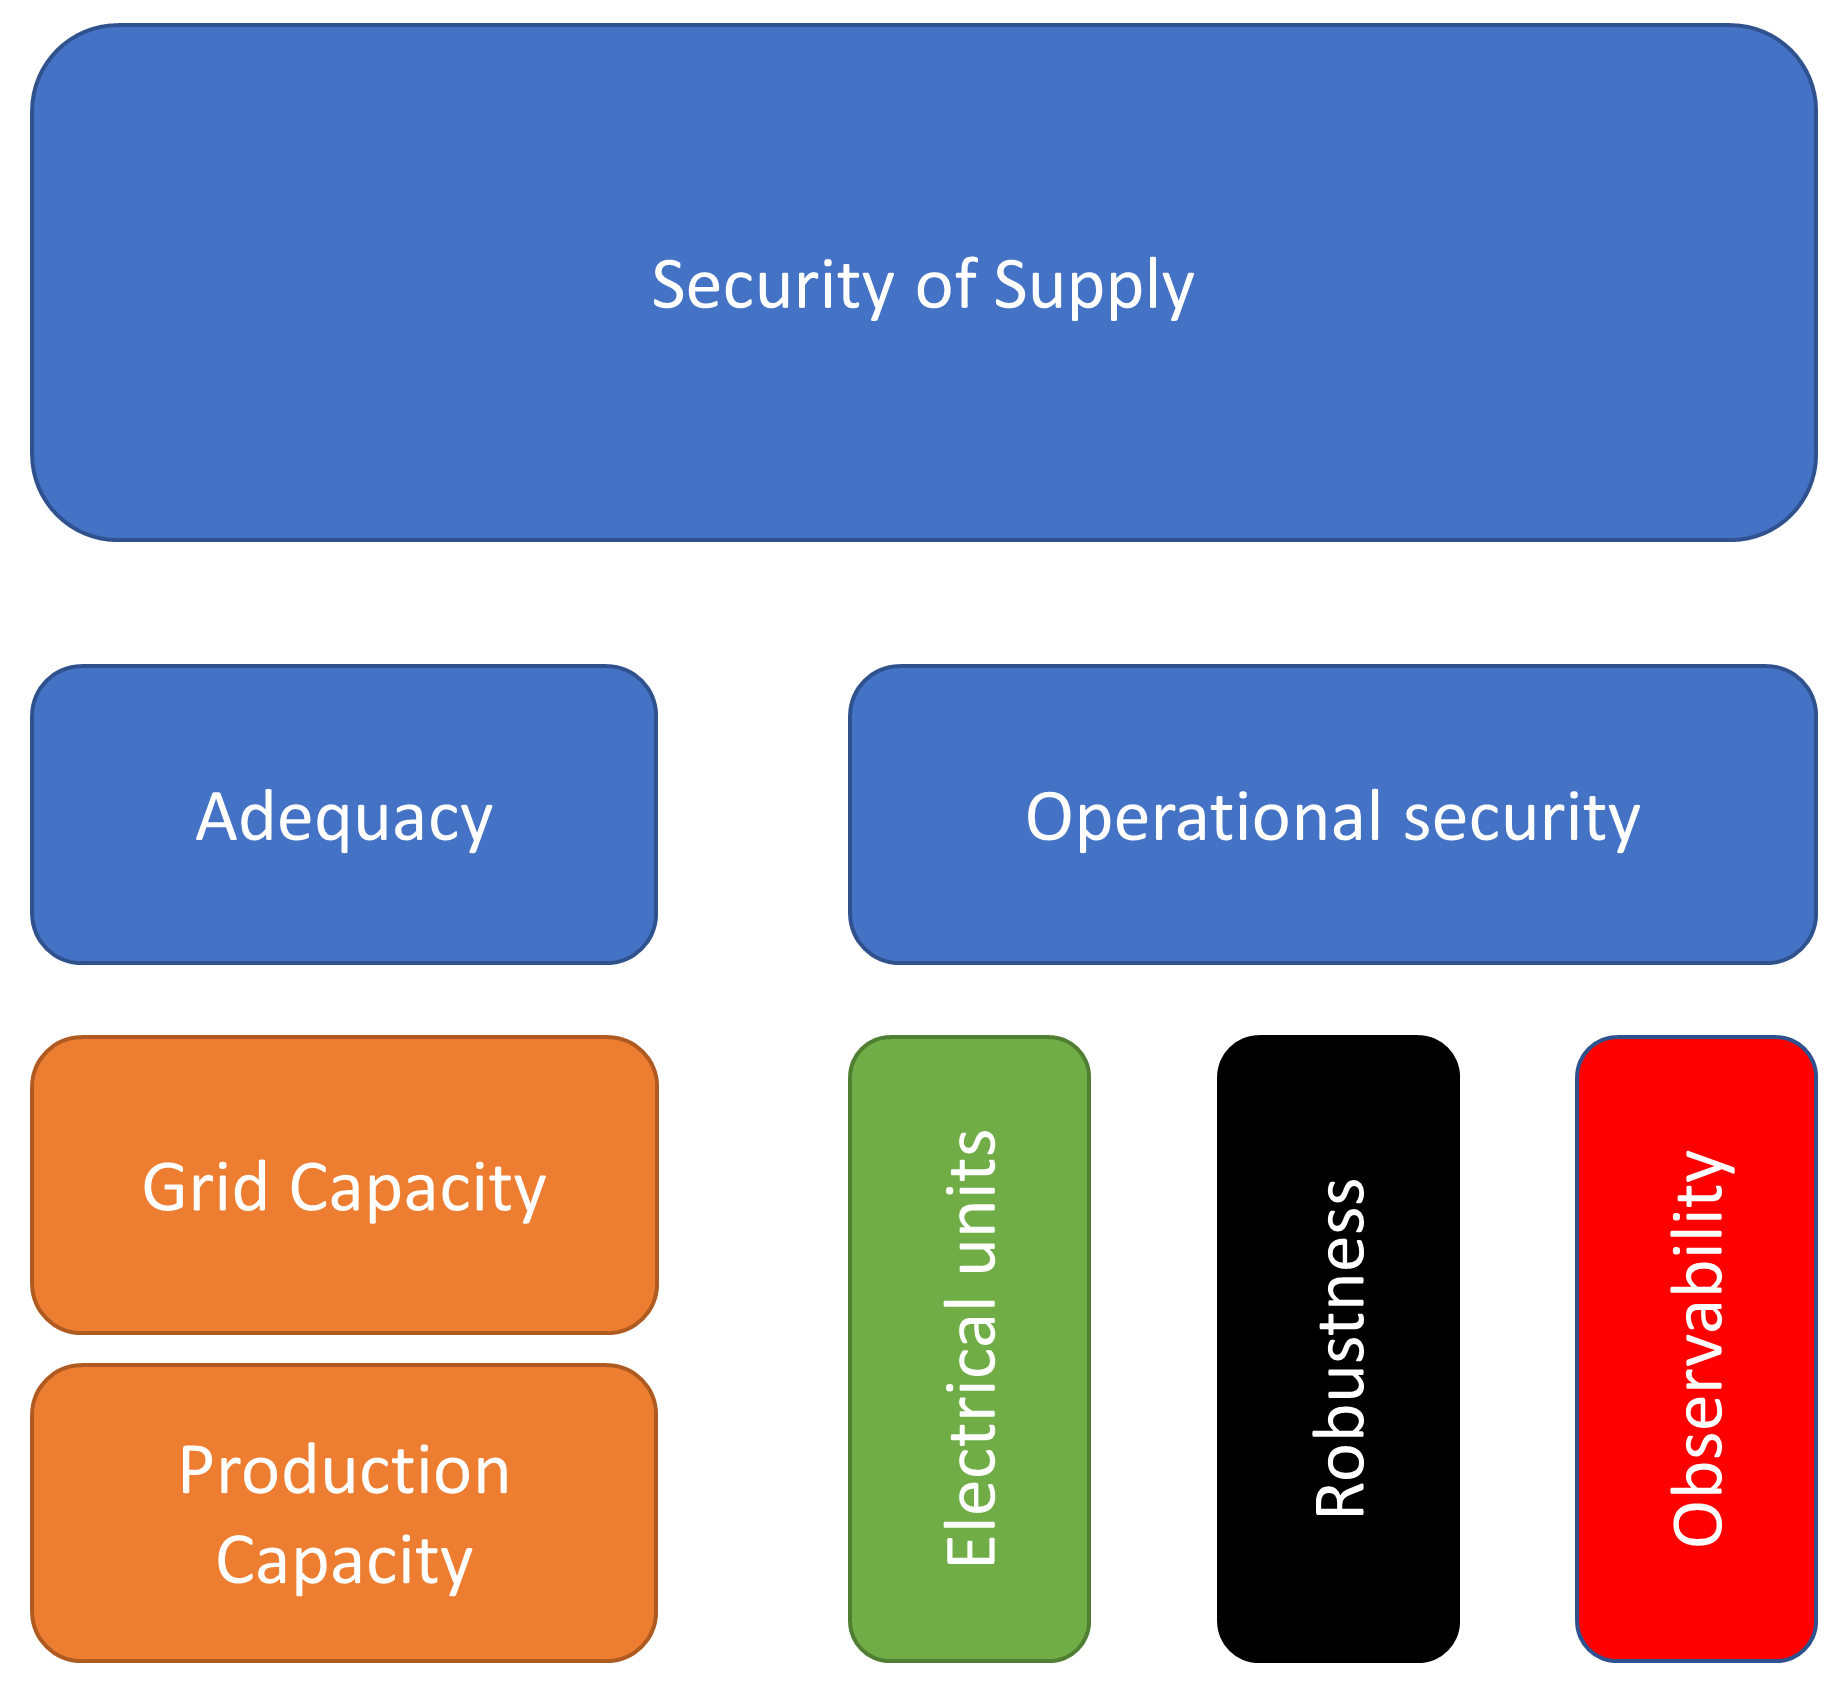
\includegraphics[scale=0.1]{Figures/TSO1.png} \end{center}}
\onslide<7->{\centering 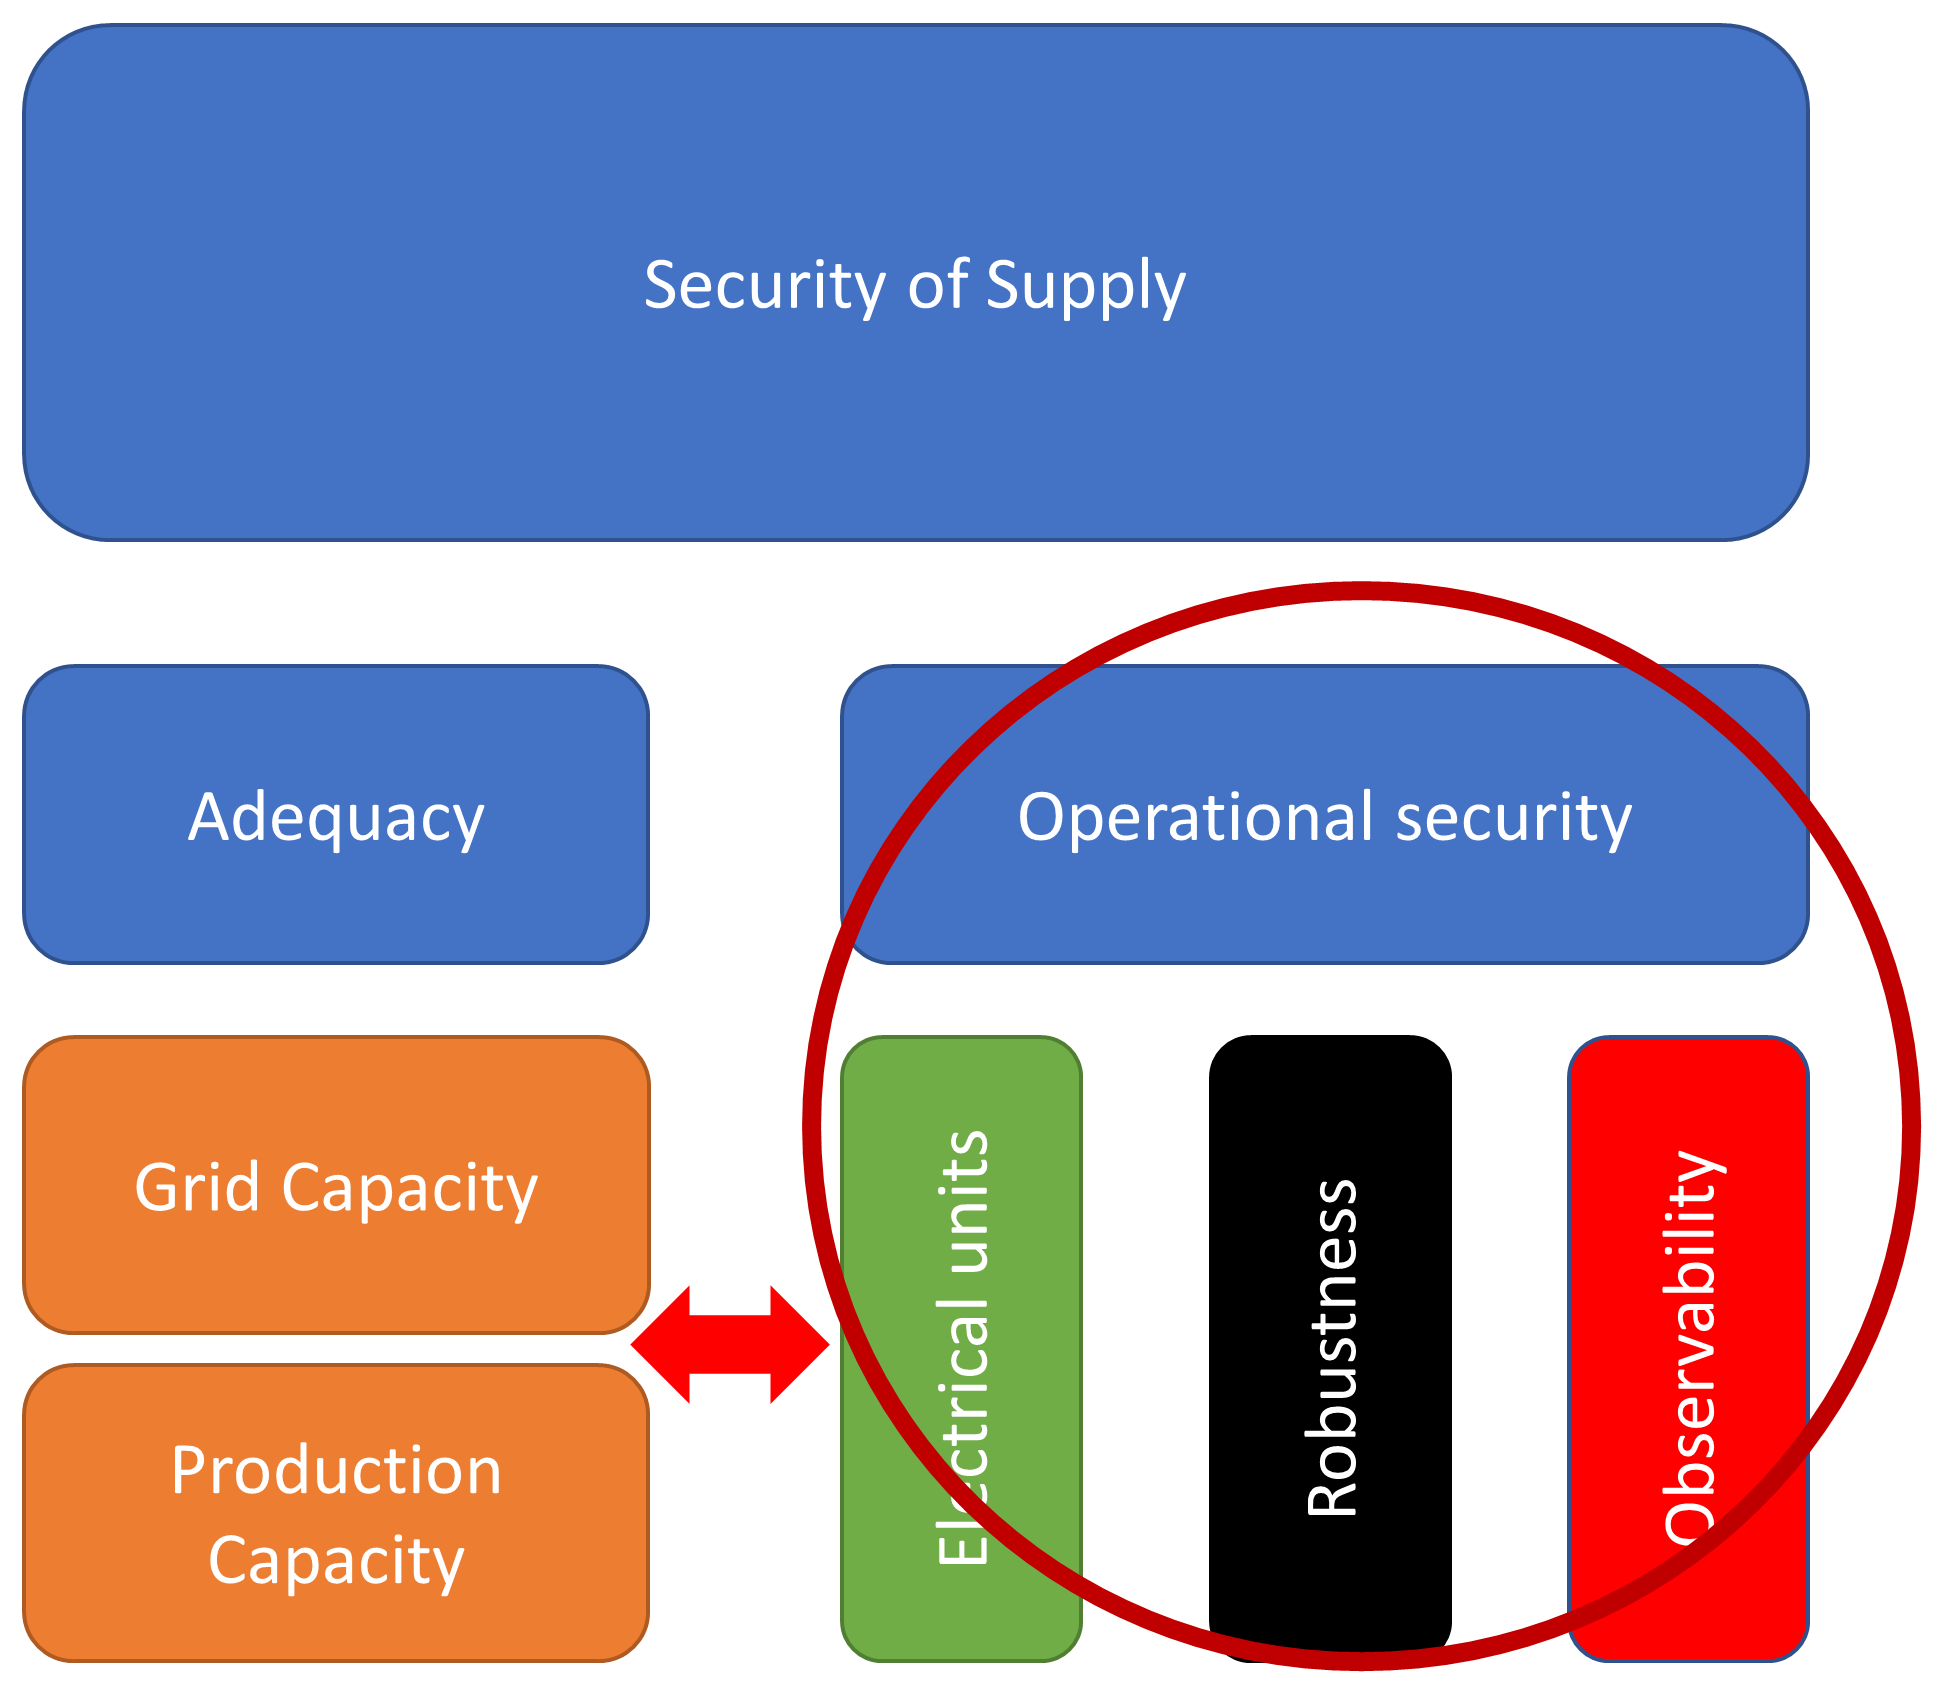
\includegraphics[scale=0.1]{Figures/TSO2.png}}
\onslide<8->{\\{\tiny System Operation shall be done to the lowest achievable costs!}}
\end{frame}
%%%%%%%%%%%%%%%%%%%%%%%%%%%%%%%%%%%%%%%%%%
%%%%%%%%%%%%%%%%%%%%%%%%%%%%%%%%%%%%%%%%%%
%%%%%%%%%%%%%%%%%%%%%%%%%%%%%%%%%%%%%%%%%%
%%%%%%%%%%%%%%%%%%%%%%%%%%%%%%%%%%%%%%%%%%
\begin{frame}{Operational Security}
\begin{itemize}
\item<1-> System challenges in the Nordic power system are changing the technical characteristics.

 \begin{columns}
    \column{0.4\textwidth}
    \begin{block}{}
Increase need of flexibility:
\end{block}
    \column{0.2\textwidth}


        \begin{alertblock}{}
        \centering
Frequency 
\end{alertblock}
\column{0.2\textwidth}
        \begin{alertblock}{}
        \centering
Voltage 
\end{alertblock}
\column{0.2\textwidth}
        \begin{alertblock}{}
        \centering
Power 
\end{alertblock}
\end{columns}
\only<1>{\centering 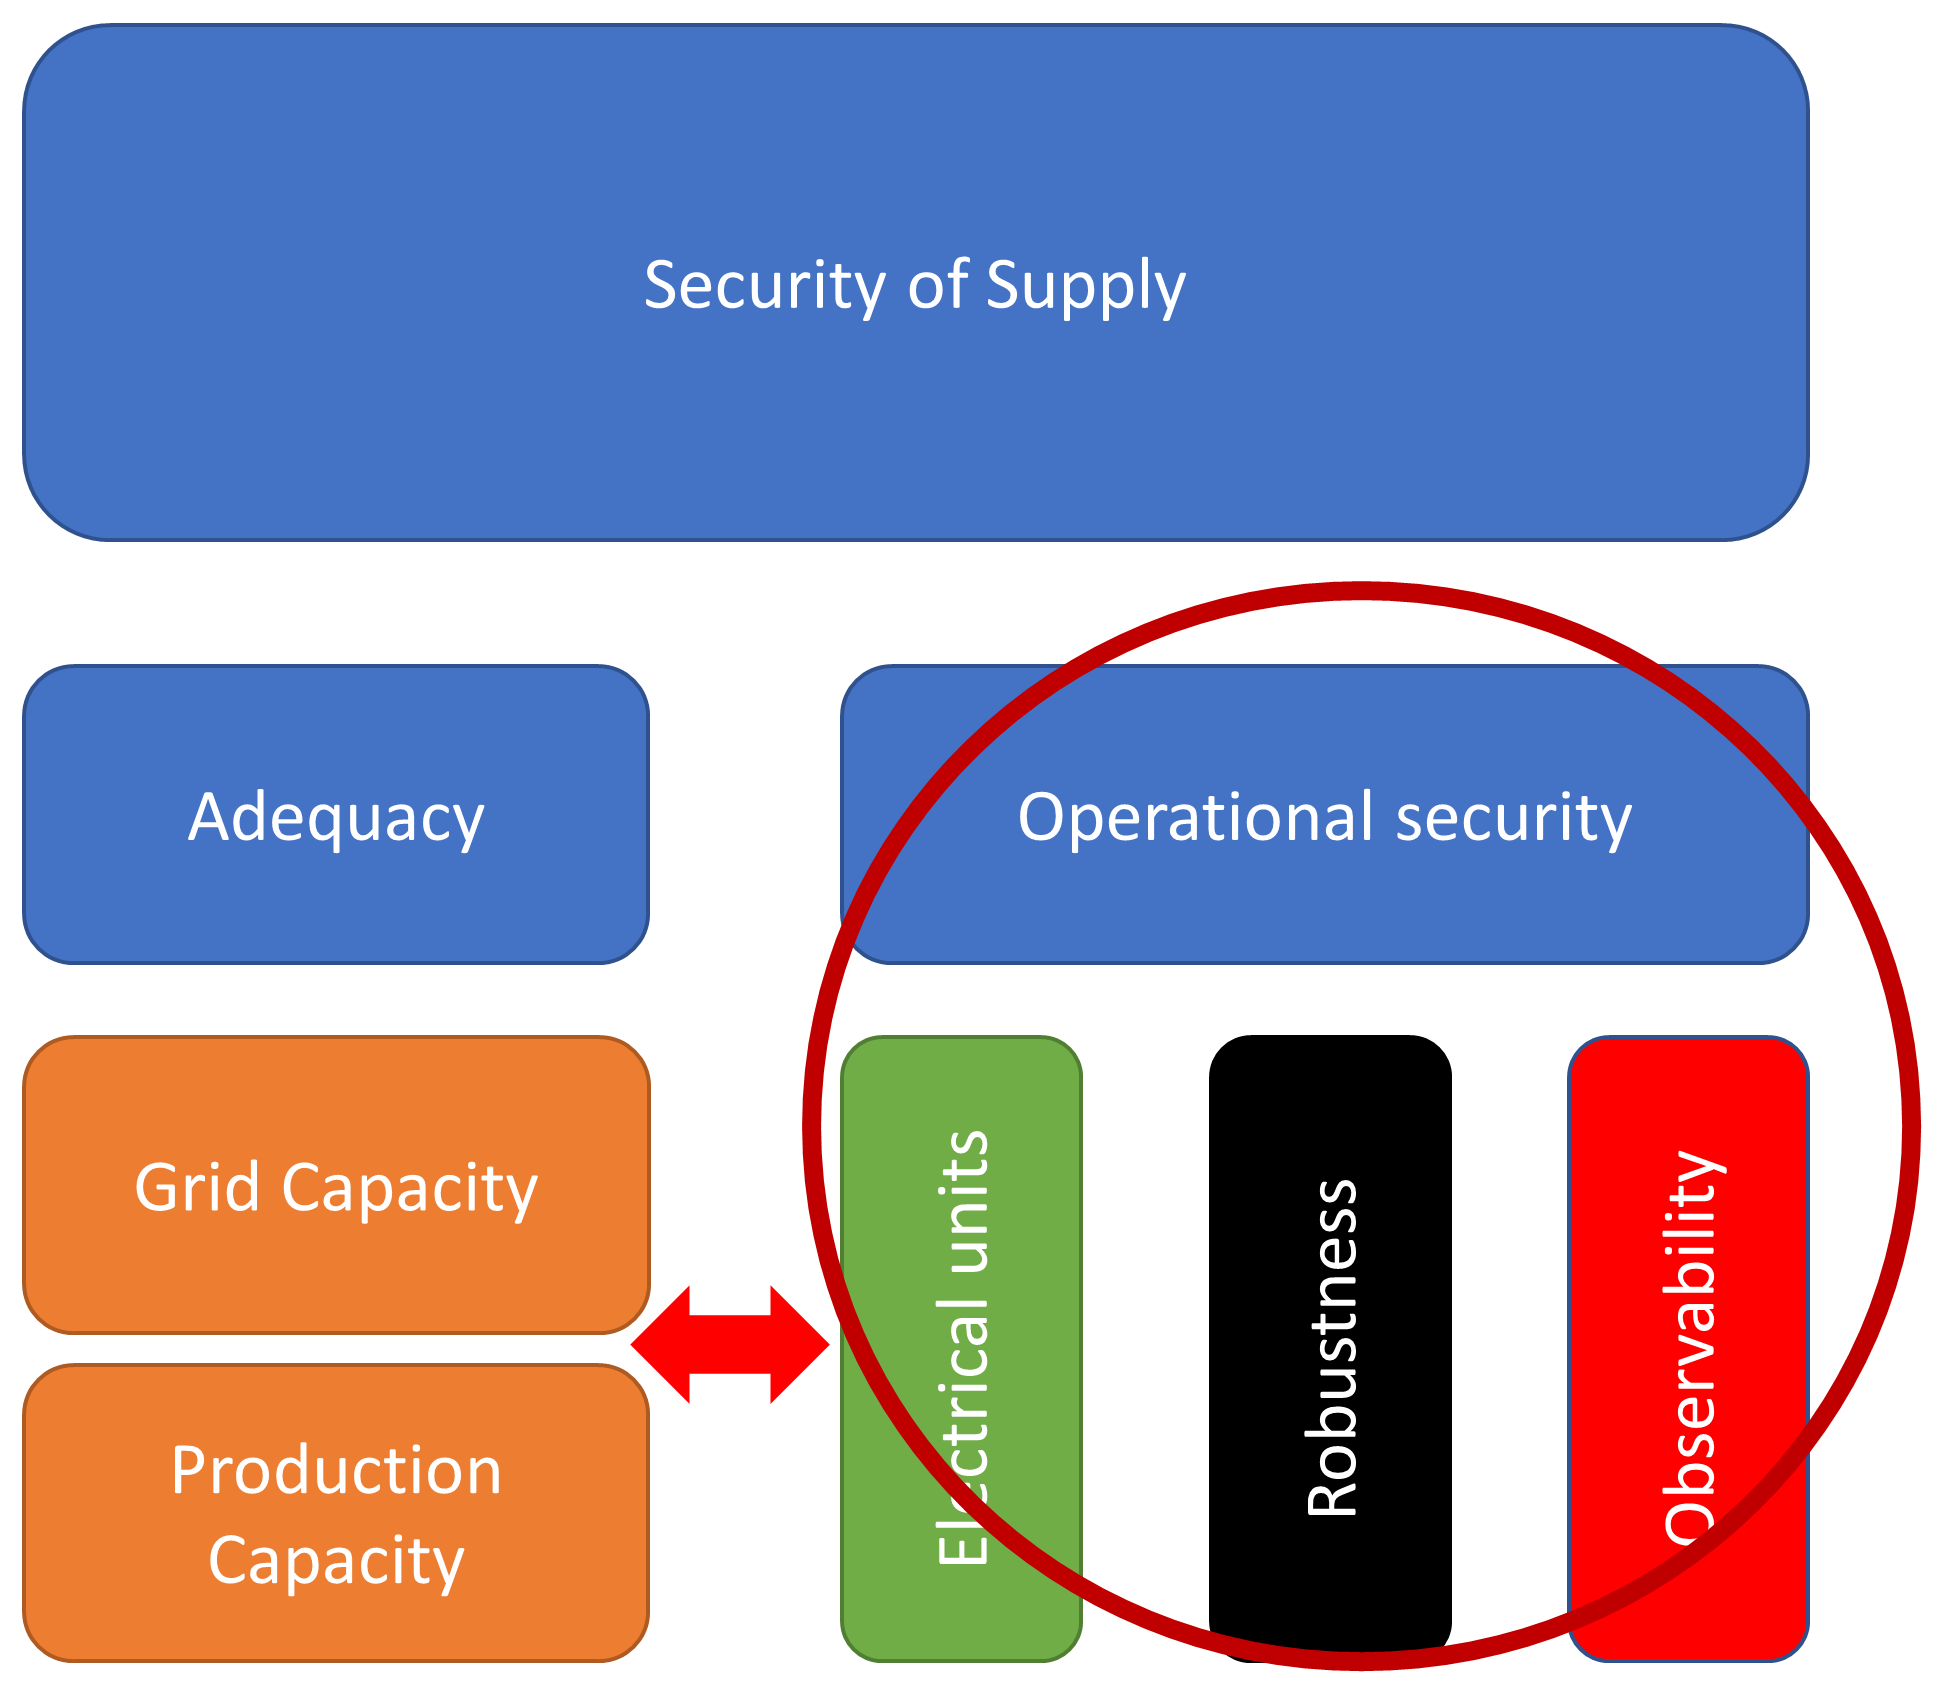
\includegraphics[scale=0.1]{Figures/TSO2.png}}
\item<2-> The system needs to adapt to the "new normal"-Flexibility is needed. \textcolor{red}{Technical abilities from all connecting parties in the system: producers, grids and
consumers.}

\only<2>{
 \begin{columns}
    \column{0.4\textwidth}
\begin{block}{New system Characteristics}

\begin{itemize}
\item Low inertia system
\item Balancing - More weather dependent power production
\end{itemize}
\end{block}    

    \column{0.2\textwidth}
\centering 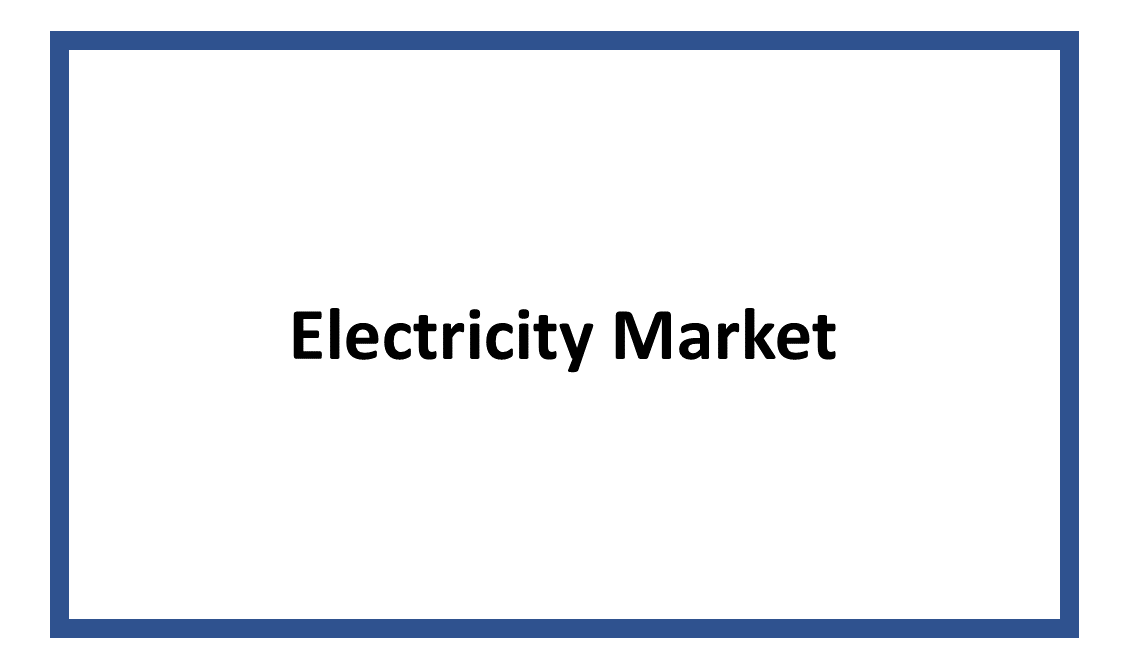
\includegraphics[scale=0.1]{Figures/FrameElecMa1.png}
\column{0.4\textwidth}
    \centering 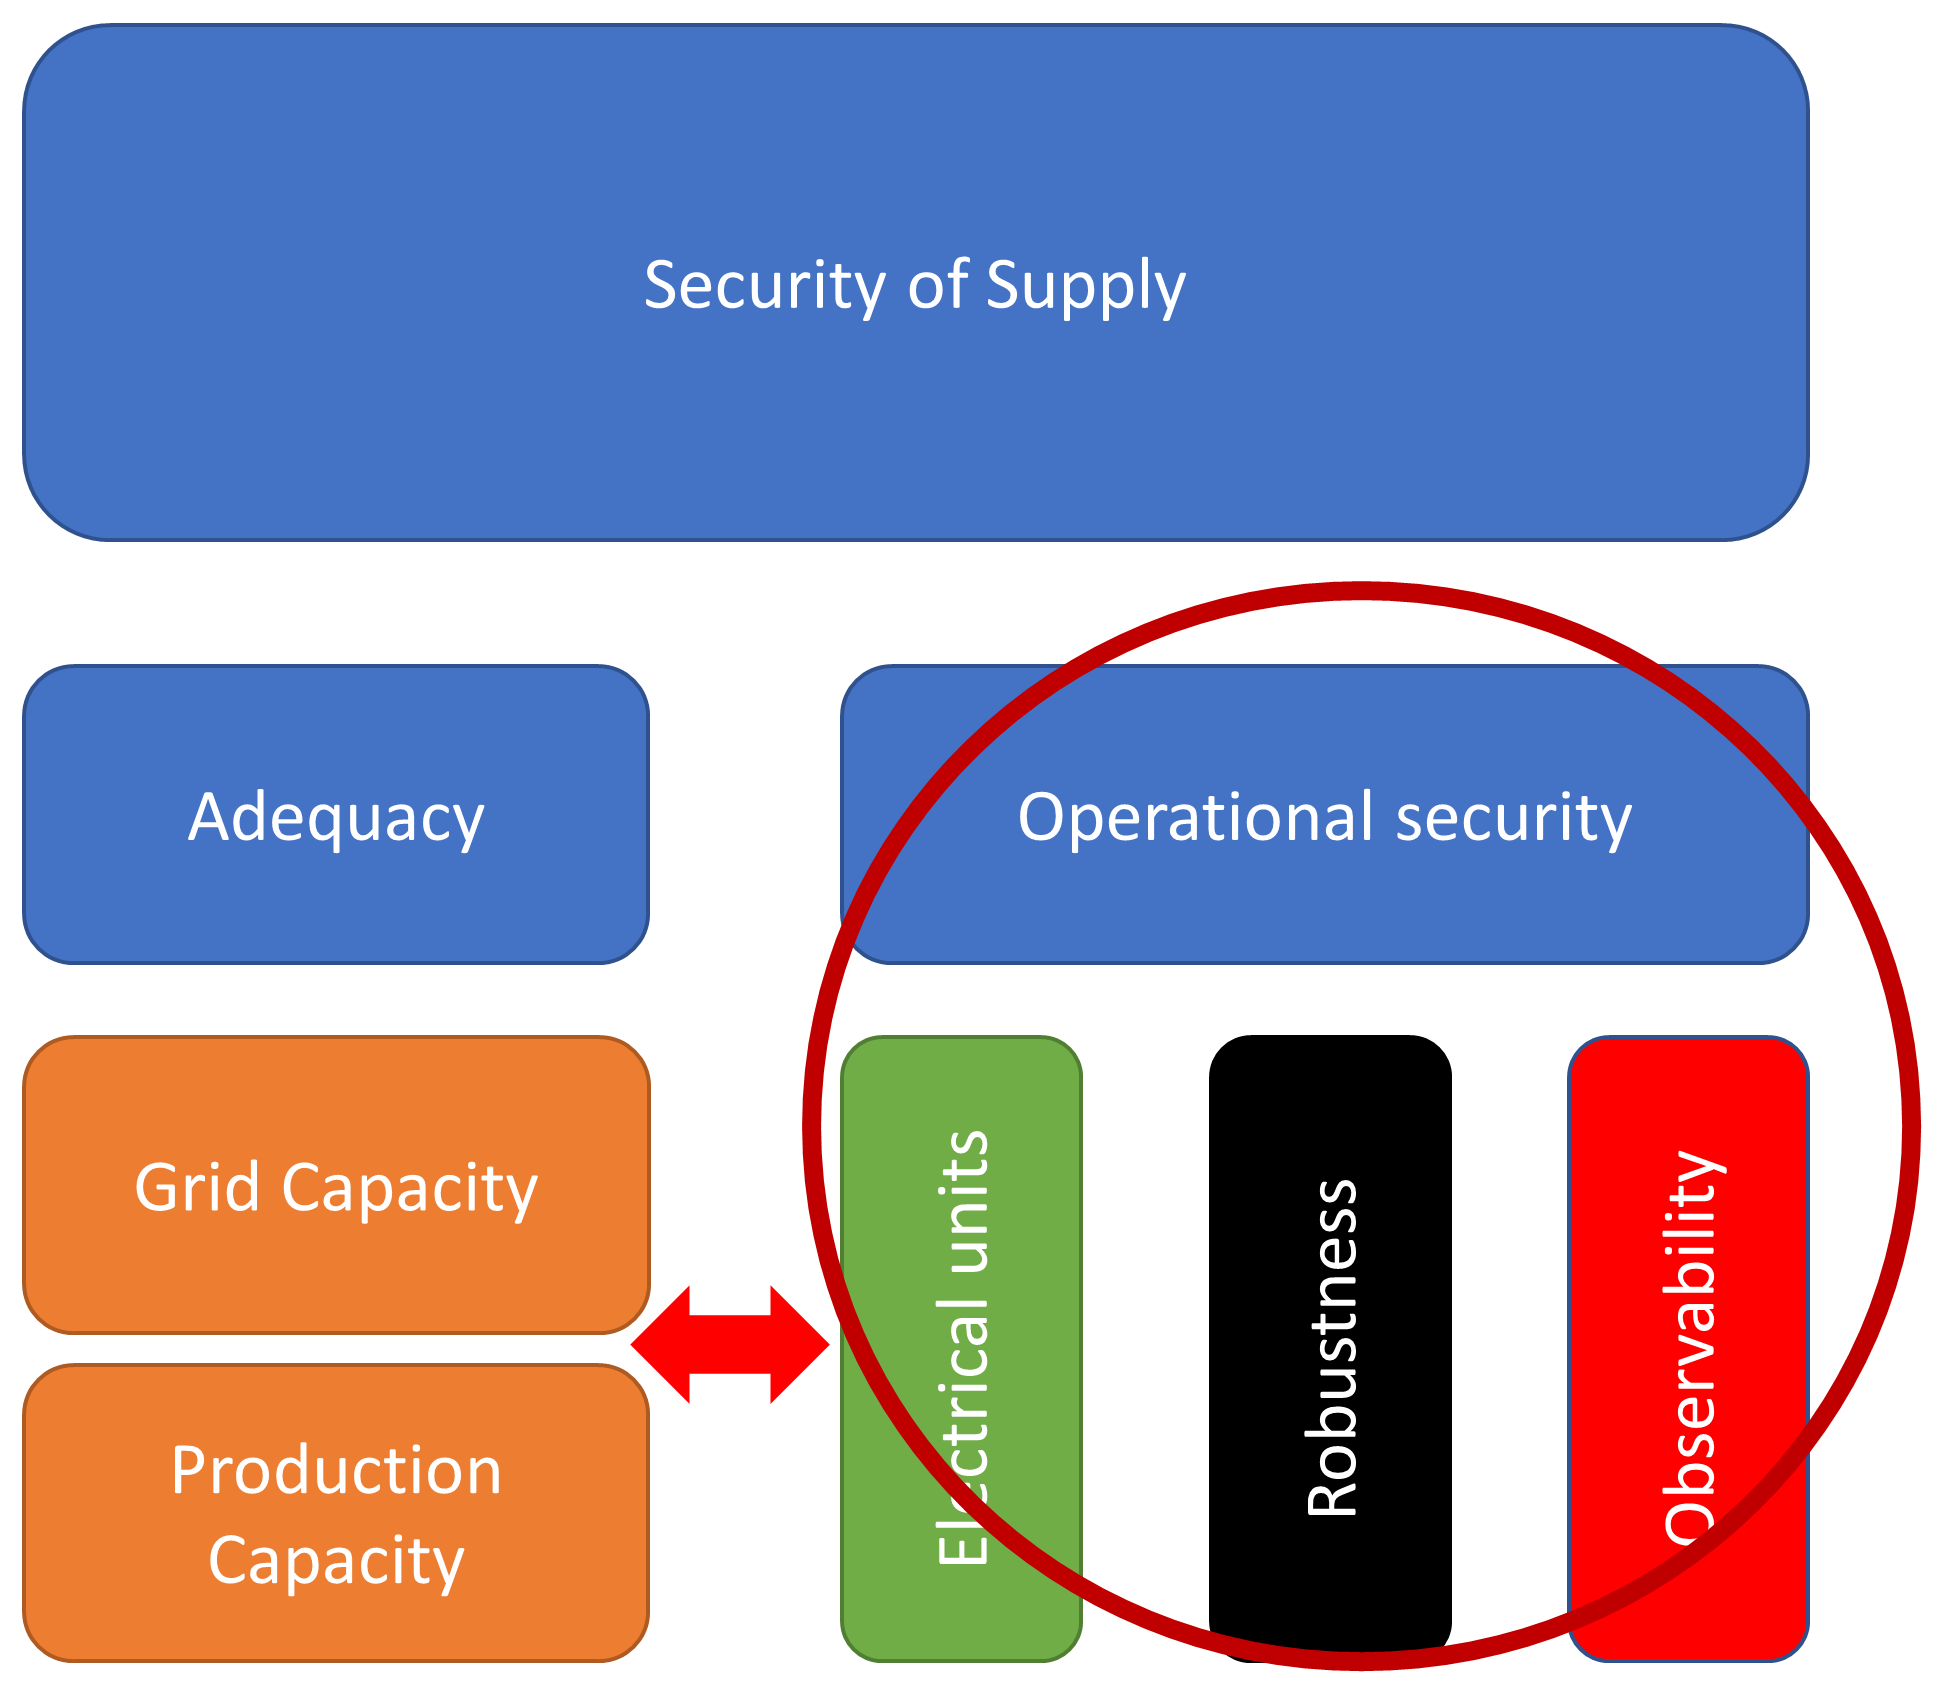
\includegraphics[scale=0.07]{Figures/TSO2.png}

\end{columns}}

\only<3>{
 \begin{columns}
    \column{0.4\textwidth}
\begin{block}{New system Characteristics}

\begin{itemize}
\item Low inertia system
\item Balancing - More weather dependent power production
\end{itemize}
\end{block}    

    \column{0.2\textwidth}
\centering 
\includegraphics[scale=0.1]{Figures/FrameElecMa2.png}
\column{0.4\textwidth}
    \centering 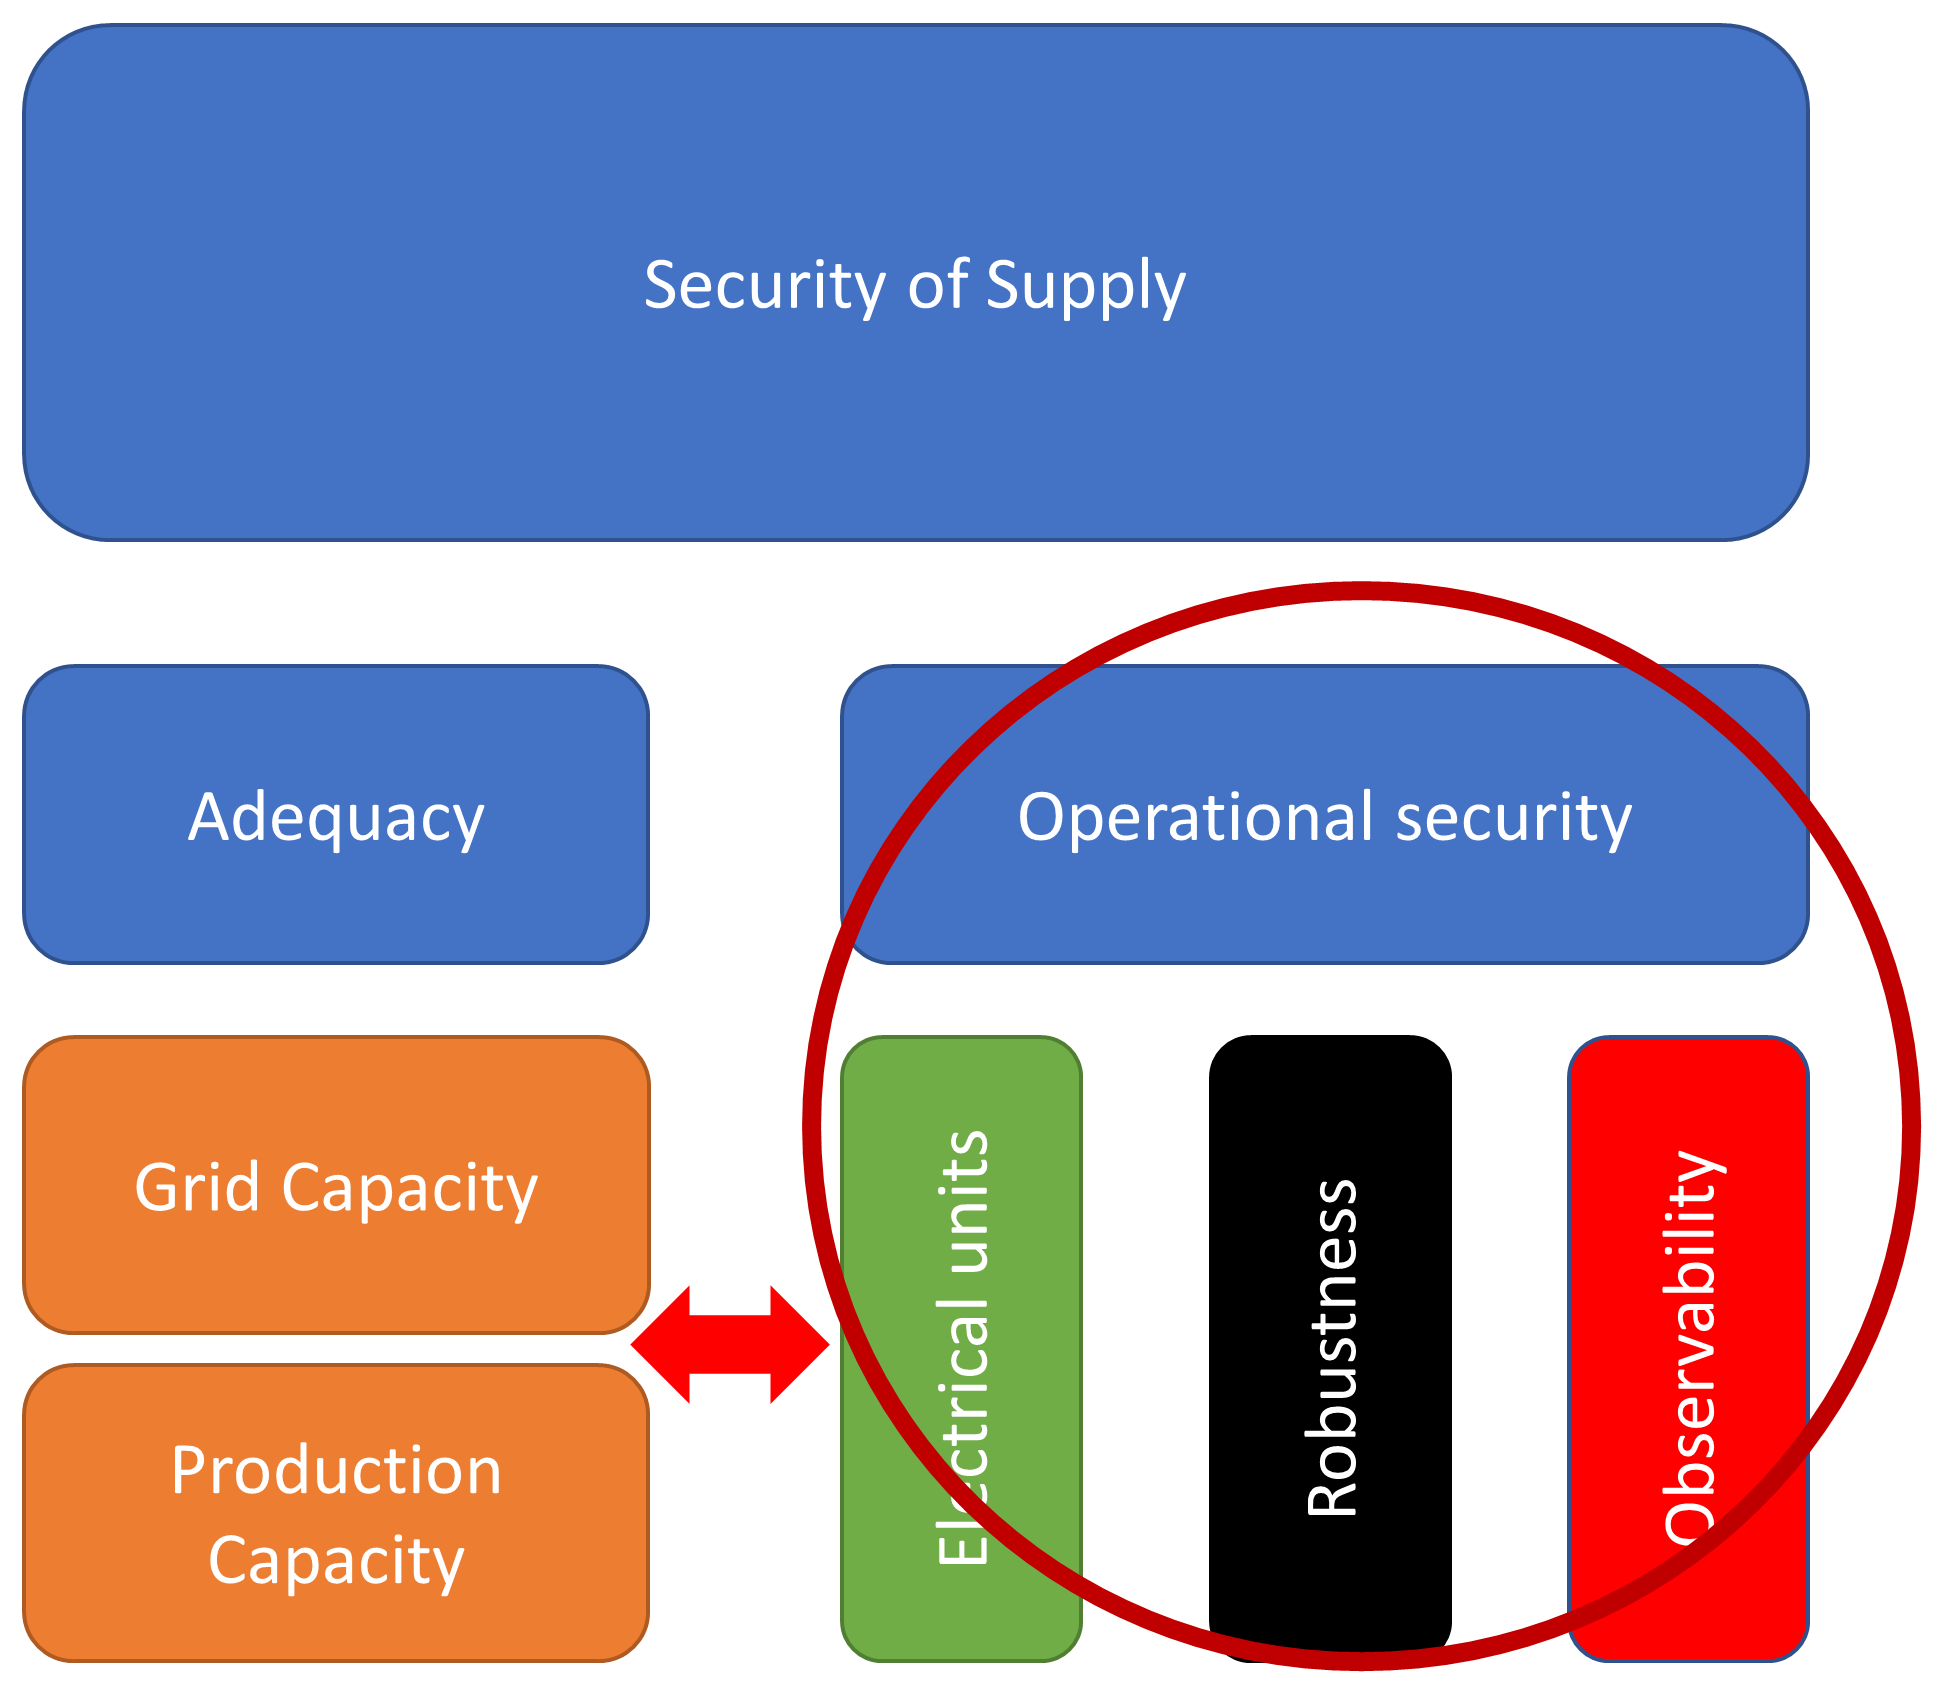
\includegraphics[scale=0.07]{Figures/TSO2.png}

\end{columns}}
\only<4>{
 \begin{columns}
    \column{0.4\textwidth}
\begin{block}{New system Characteristics}

\begin{itemize}
\item Low inertia system
\item Balancing - More weather dependent power production
\end{itemize}
\end{block}    

    \column{0.2\textwidth}
\centering 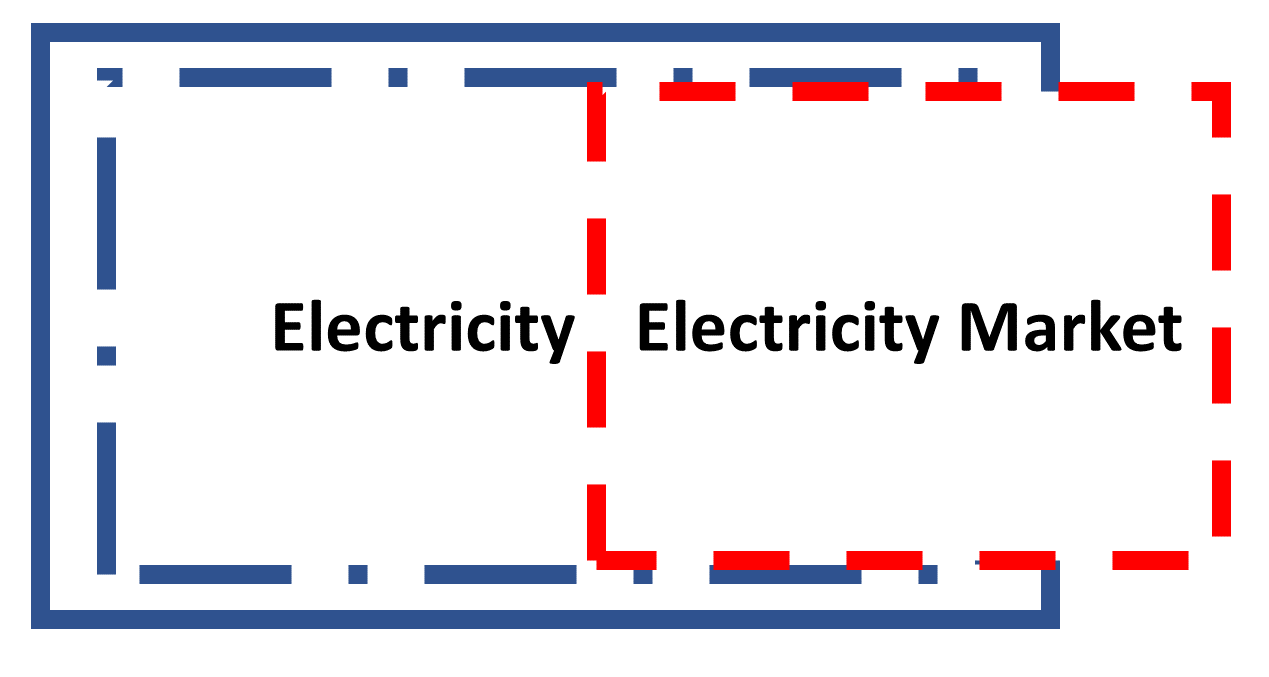
\includegraphics[scale=0.1]{Figures/FrameElecMa3.png}
\column{0.4\textwidth}
    \centering 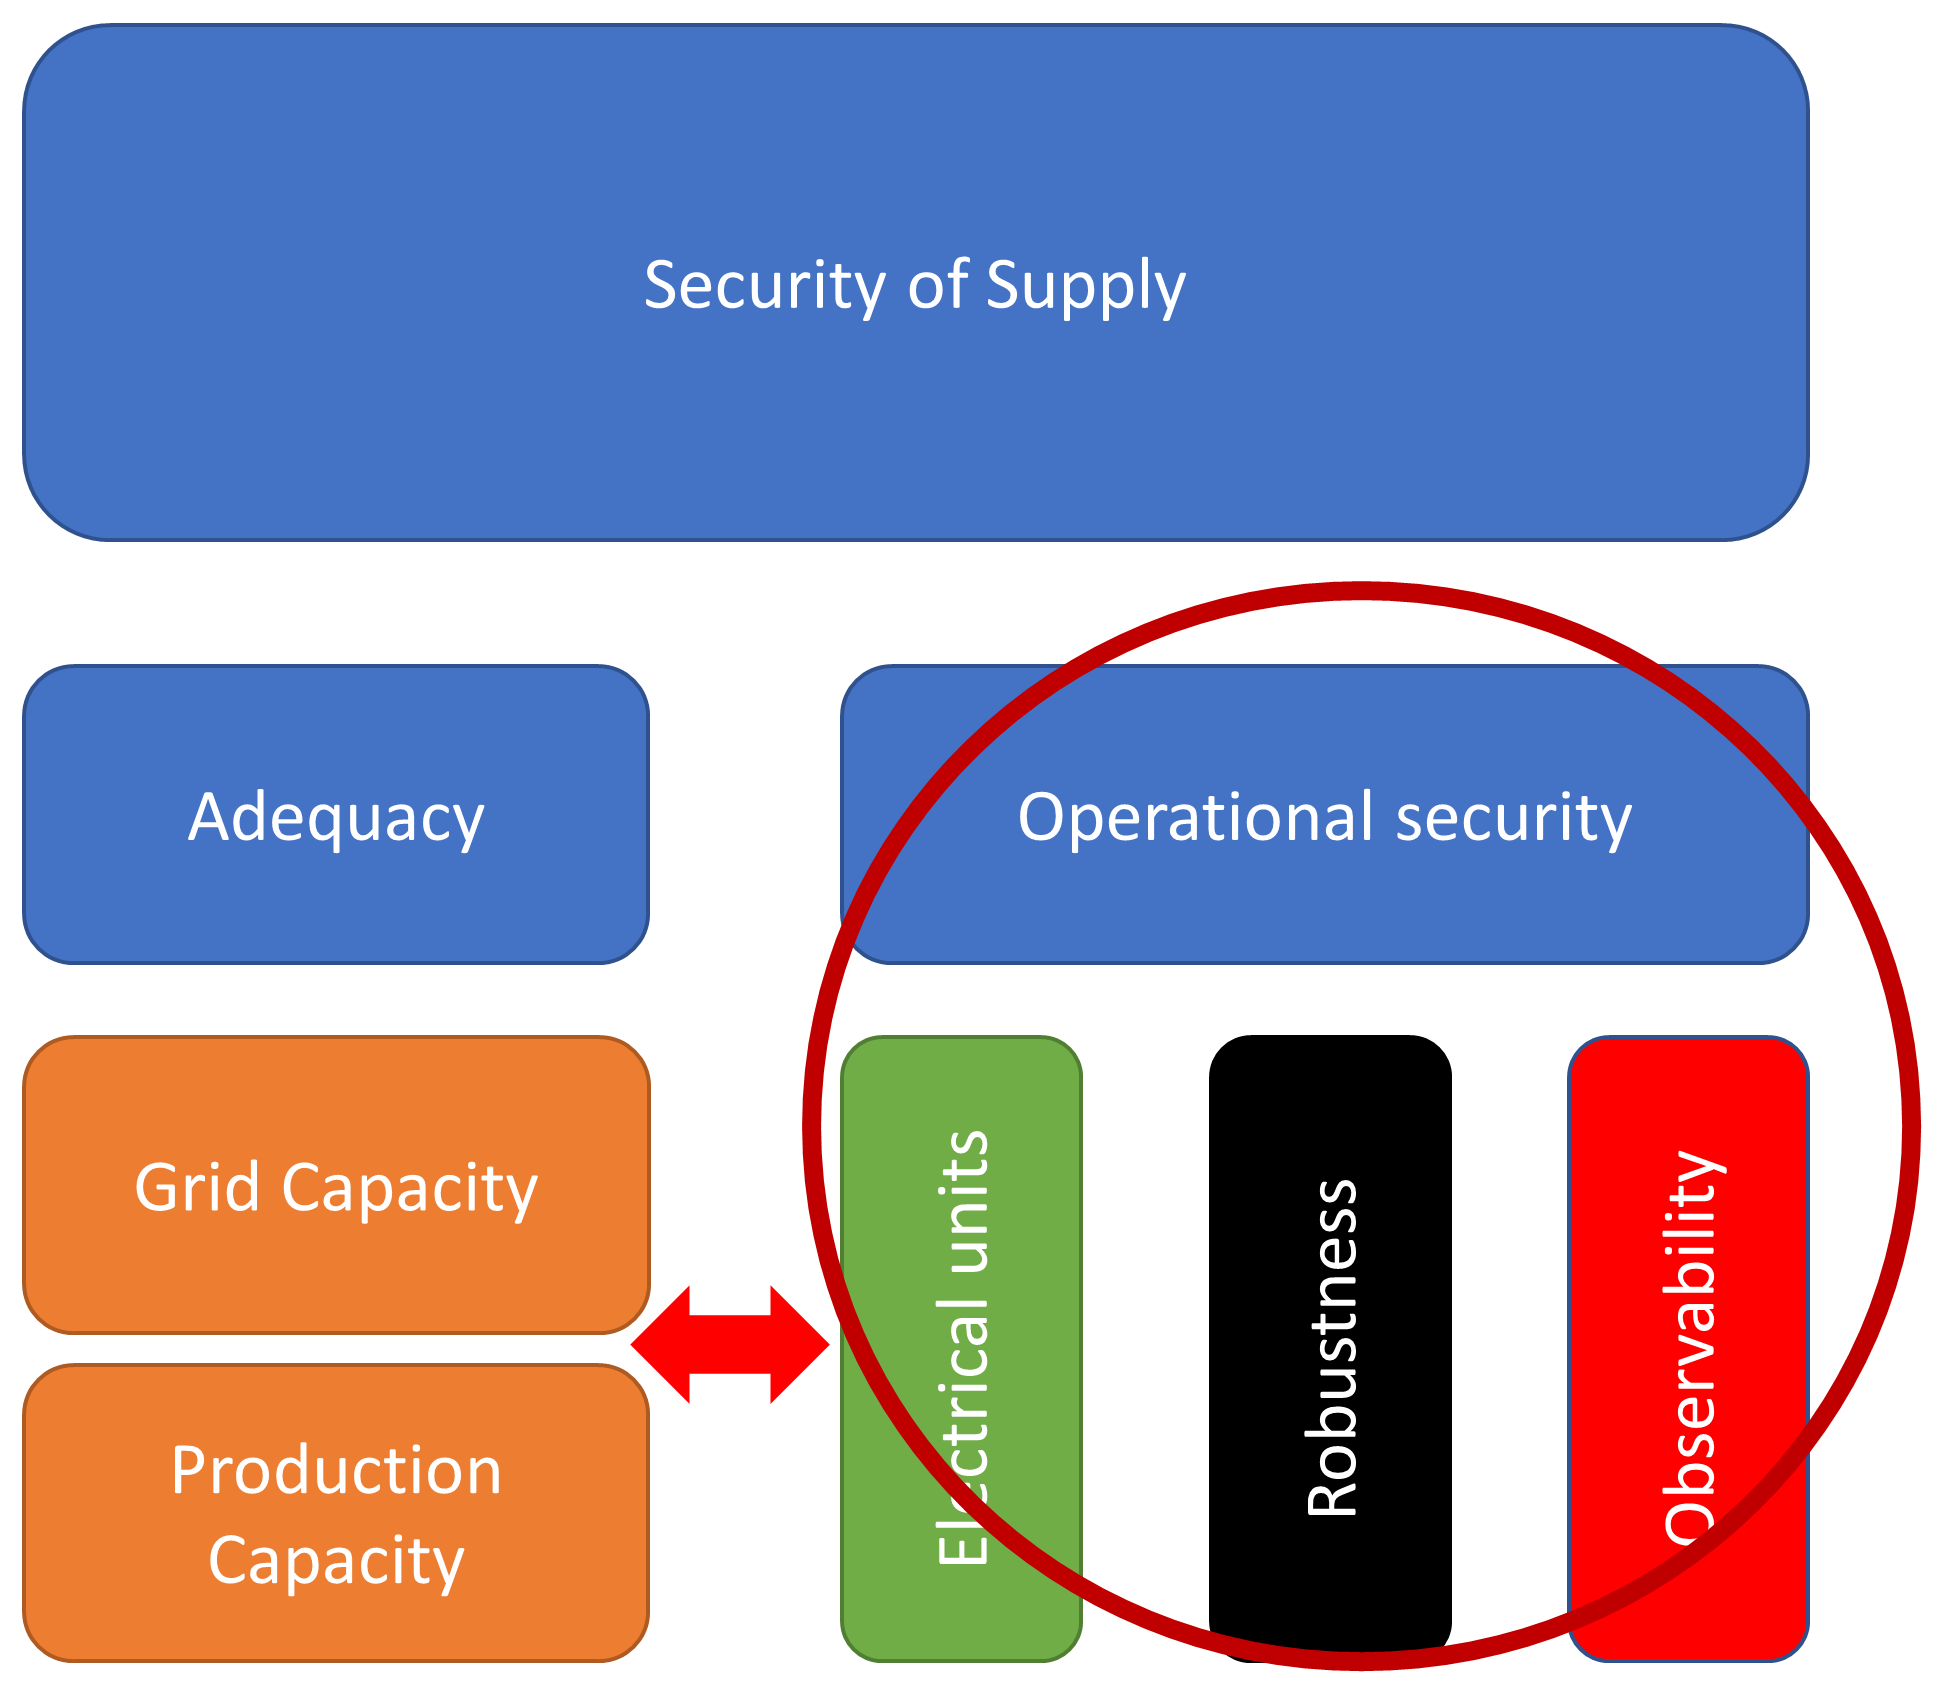
\includegraphics[scale=0.07]{Figures/TSO2.png}
\end{columns}}
\end{itemize}
\end{frame}

%%%%%%%%%%%%%%%%%%%%%%%%%%%%%%%%%%%%%%%%%%
%%%%%%%%%%%%%%%%%%%%%%%%%%%%%%%%%%%%%%%%%%
%%%%%%%%%%%%%%%%%%%%%%%%%%%%%%%%%%%%%%%%%%
%%%%%%%%%%%%%%%%%%%%%%%%%%%%%%%%%%%%%%%%%%
\begin{frame}{From A to B}
\centering 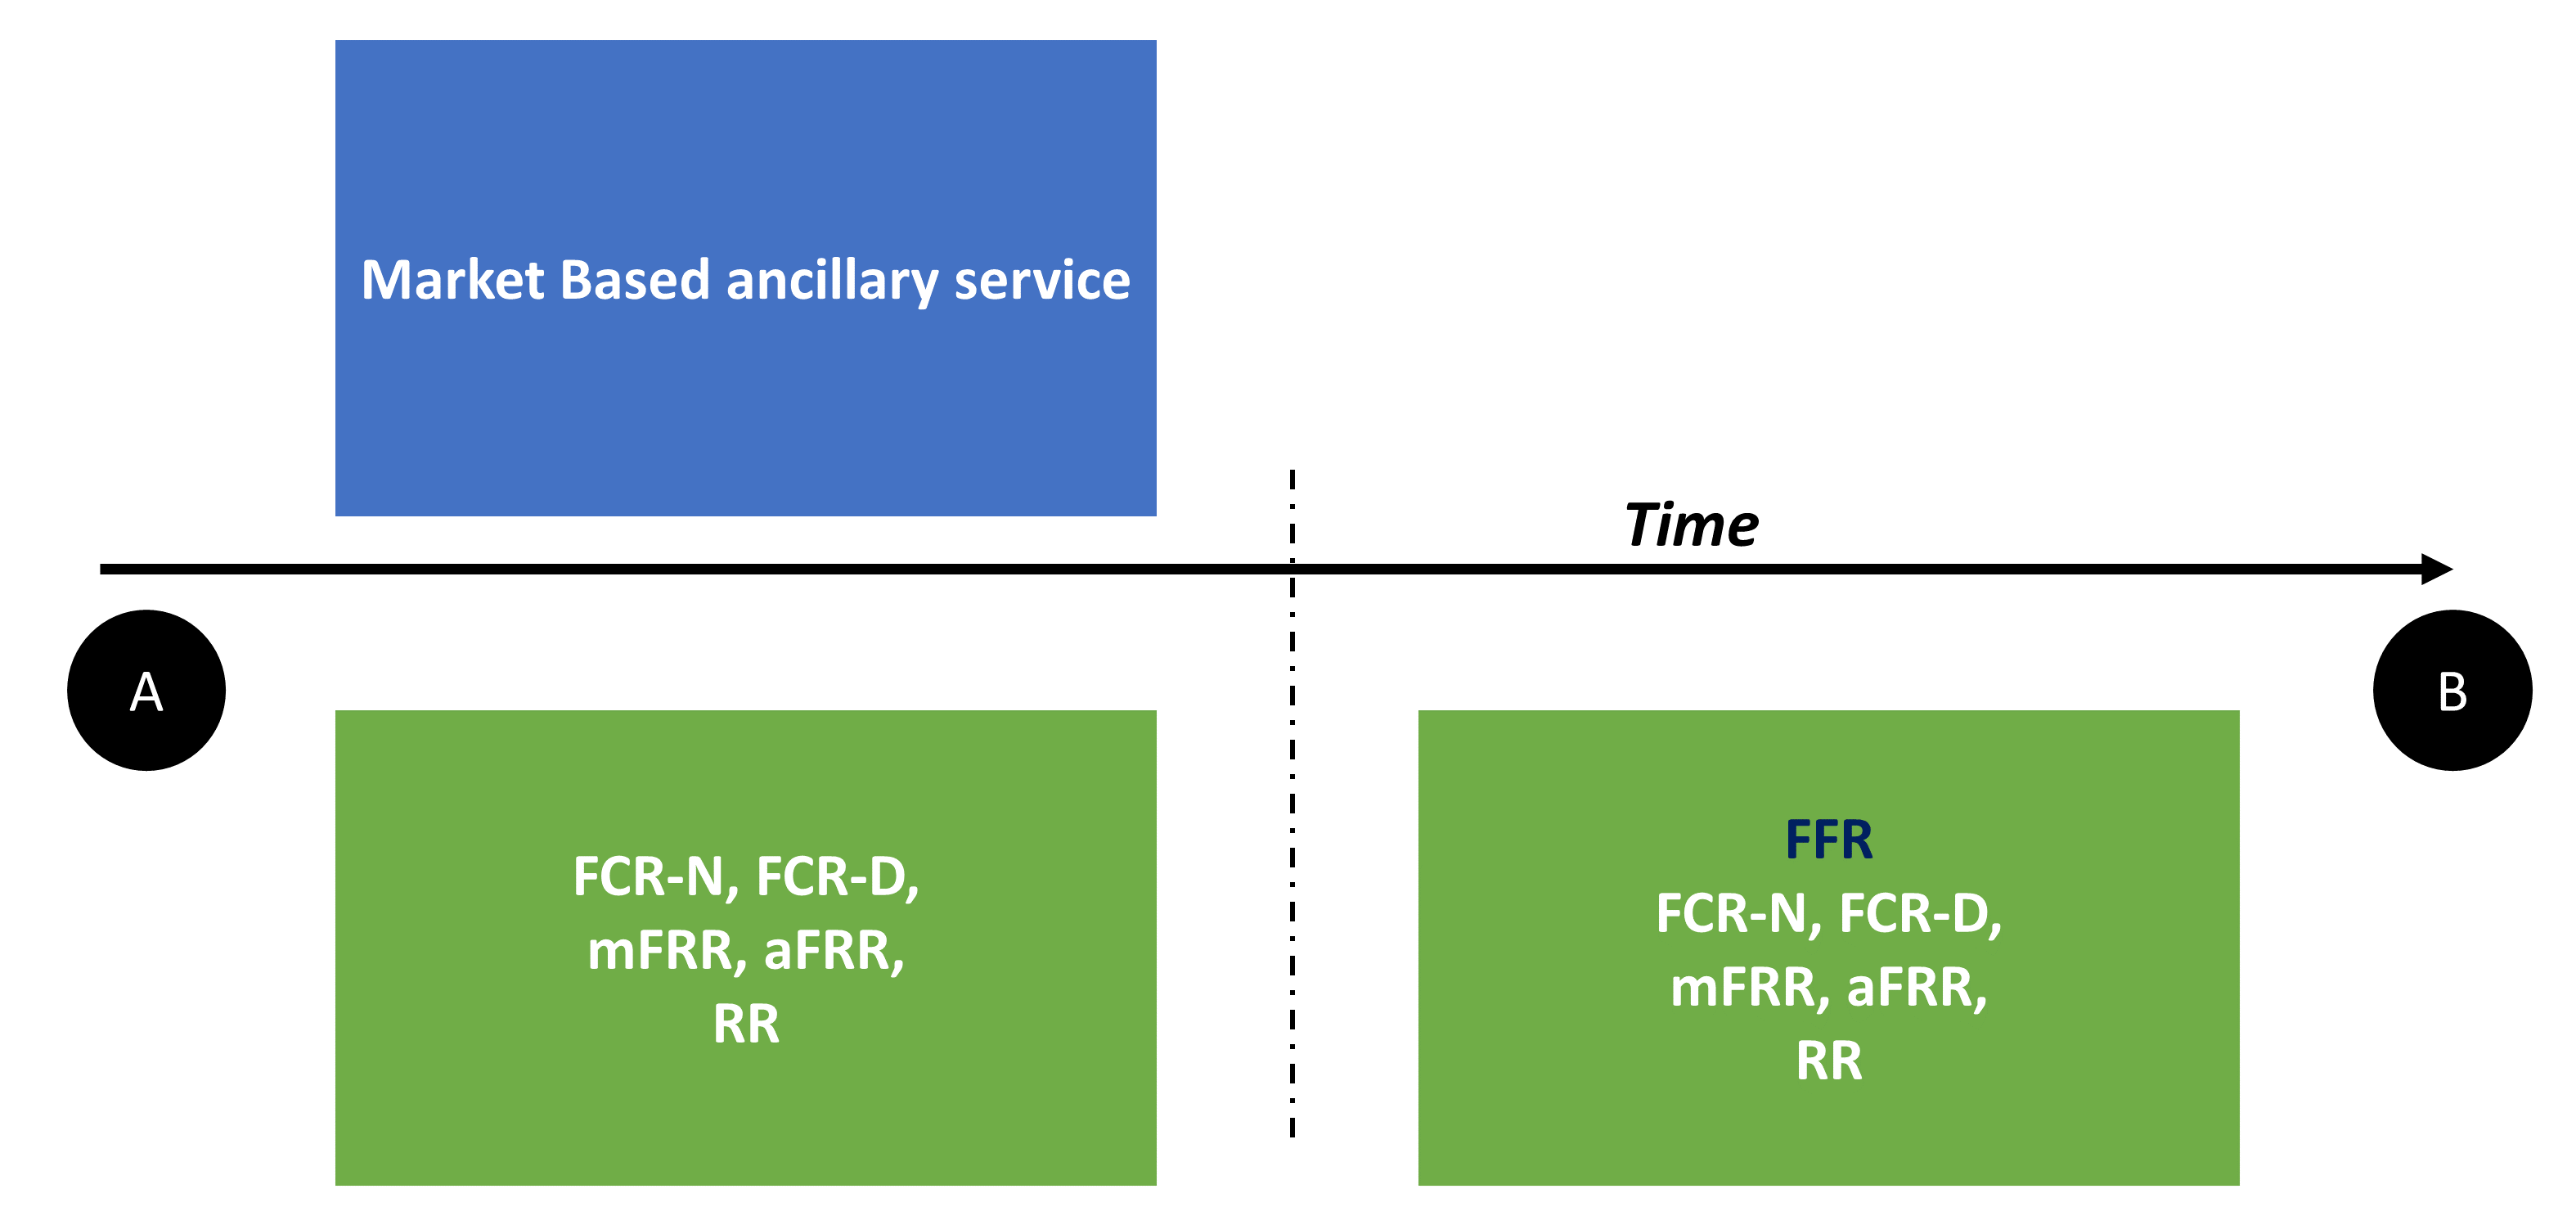
\includegraphics[scale=0.13]{Figures/TimeEvolutionFFR.png}
\onslide<1-> {\begin{block}{}
why do we want market based solution?
\end{block} }
\onslide<2-> {\begin{alertblock}{}
Because we want to make sure who knows each power plant the best, put in a bid when suits them. 
\end{alertblock} }
\end{frame}

%%%%%%%%%%%%%%%%%%%%%%%%%%%%%%%%%%%%%%%%%%
%%%%%%%%%%%%%%%%%%%%%%%%%%%%%%%%%%%%%%%%%%
%%%%%%%%%%%%%%%%%%%%%%%%%%%%%%%%%%%%%%%%%%
%%%%%%%%%%%%%%%%%%%%%%%%%%%%%%%%%%%%%%%%%%

\begin{frame}
\begin{figure}
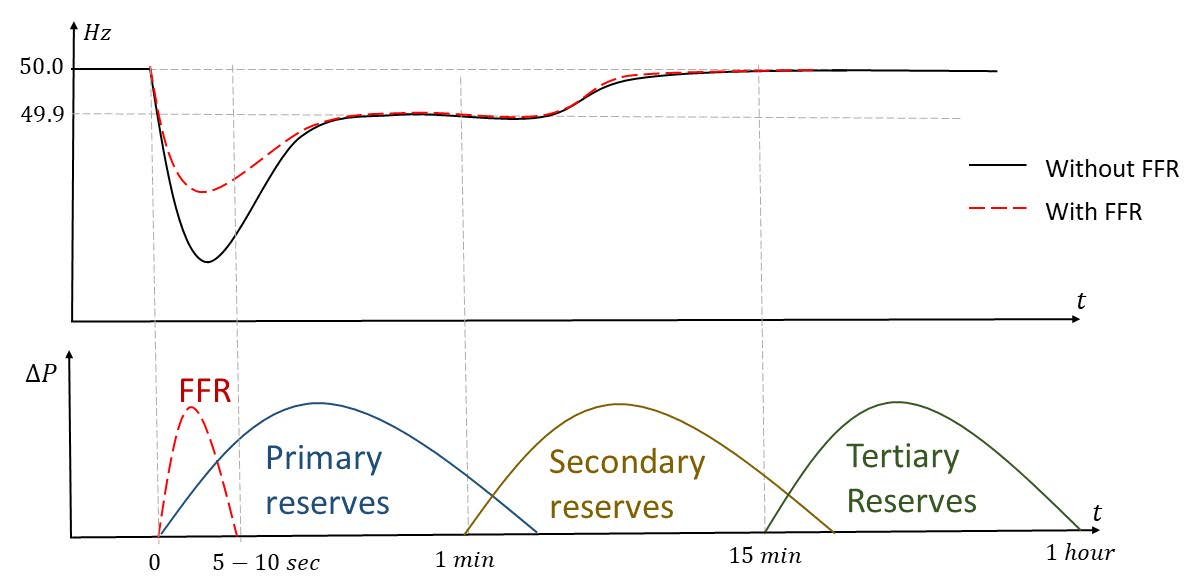
\includegraphics[scale=1.5]{Figures/FFR1.jpg}
\caption{Power system frequency response to a power deficit \textcolor{gray}{\tiny [Kjetil Uhlen and Olav Bjarte Fosso. Power system operation and Frequency control
(lecture notes).]}}
\end{figure}
\end{frame}

%%%%%%%%%%%%%%%%%%%%%%%%%%%%%%%%%%%%%%%%%%
%%%%%%%%%%%%%%%%%%%%%%%%%%%%%%%%%%%%%%%%%%
%%%%%%%%%%%%%%%%%%%%%%%%%%%%%%%%%%%%%%%%%%
%%%%%%%%%%%%%%%%%%%%%%%%%%%%%%%%%%%%%%%%%%
\begin{frame}{Justification-Why do we need FFR?}
\begin{block}{Frequency stability in Nordic system}
Frequency stability here mainly referred to the ability of securing the frequency above a threshold
\end{block}

\begin{enumerate}

\item<1-> The current response of the primary frequency reserve in the Nordic synchronous area does not ensure frequency stability in low inertia situation. \footnote{{\tiny[entsoe, "Fast frequency reserve-solution to the Nordic inertia challenge" 2019]}}
\item<2->  The volume needed to affect the minimum frequency by 0.1 in an 80 GWs system is 20 GWs \footnote{{\tiny[Ørum et al., Future system inertia 2, 2017]}}. The availability of different possible techniques are varies but the cost will be high.  
\item<3-> FFR is deemed the most promising mitigation solution for low inertia situation since several techniques can provide fast power response estimated at low socio-economic costs, either as a disconnection of load or fast increase from inverter-based generation and storage  \footnote{{\tiny[M. Kuivaniemi and E. A. Jansson, "FFR feasibility study," Unpublished report, 2019]}} 
\end{enumerate}
\end{frame}

%%%%%%%%%%%%%%%%%%%%%%%%%%%%%%%%%%%%%%%%%%
%%%%%%%%%%%%%%%%%%%%%%%%%%%%%%%%%%%%%%%%%%
%%%%%%%%%%%%%%%%%%%%%%%%%%%%%%%%%%%%%%%%%%
%%%%%%%%%%%%%%%%%%%%%%%%%%%%%%%%%%%%%%%%%%
\begin{frame}{Nordic TSOs: Inertia Forecasting}
\onslide<1-> {\textcolor{blue}{\textbf{> \ Inertia Monitoring:}} {\scriptsize Real time kinetic energy estimation tool is implemented for all Nordic TSOs, in their supervisory control and data acquisition SCADA/Energy Managment System (EMS).\\}}
\only<1>{ \centering
\begin{figure}
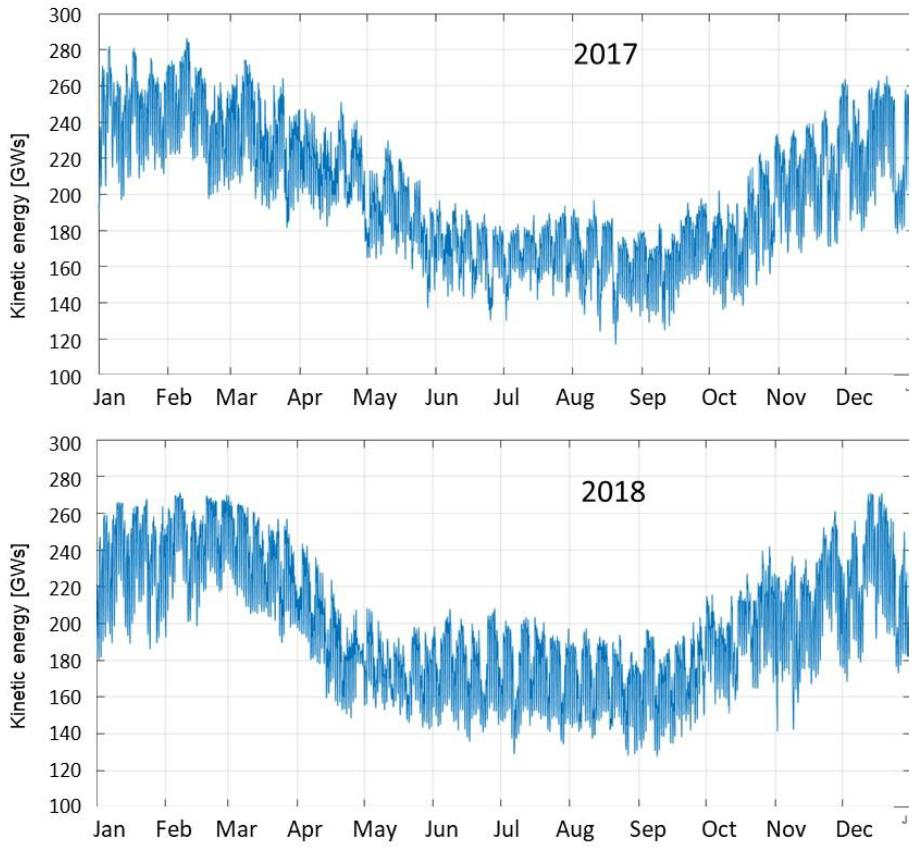
\includegraphics[scale=0.4]{Figures/FFREstimate1.jpg}
\caption{\tiny Estimated kinetic values (Nordic synchronous system)
}\end{figure}}
\onslide<2->{\textcolor{blue}{\textbf{> \ Inertia Forecasting:}} {\scriptsize The aim of forecasting the system inertia  is to estimate the instantaneous frequency minimum for the online reference incident.\\}}
\onslide<3->{\textcolor{blue}{\textbf{> \ FFR estimate need:}} {\scriptsize see [“Fast Frequency Reserve – Solution to the Nordic inertia challenge ” by entsoe]} }
		\vskip -0.7cm

\only<3>{
\begin{columns}
    \column{0.5\textwidth}
 \centering
\begin{figure}
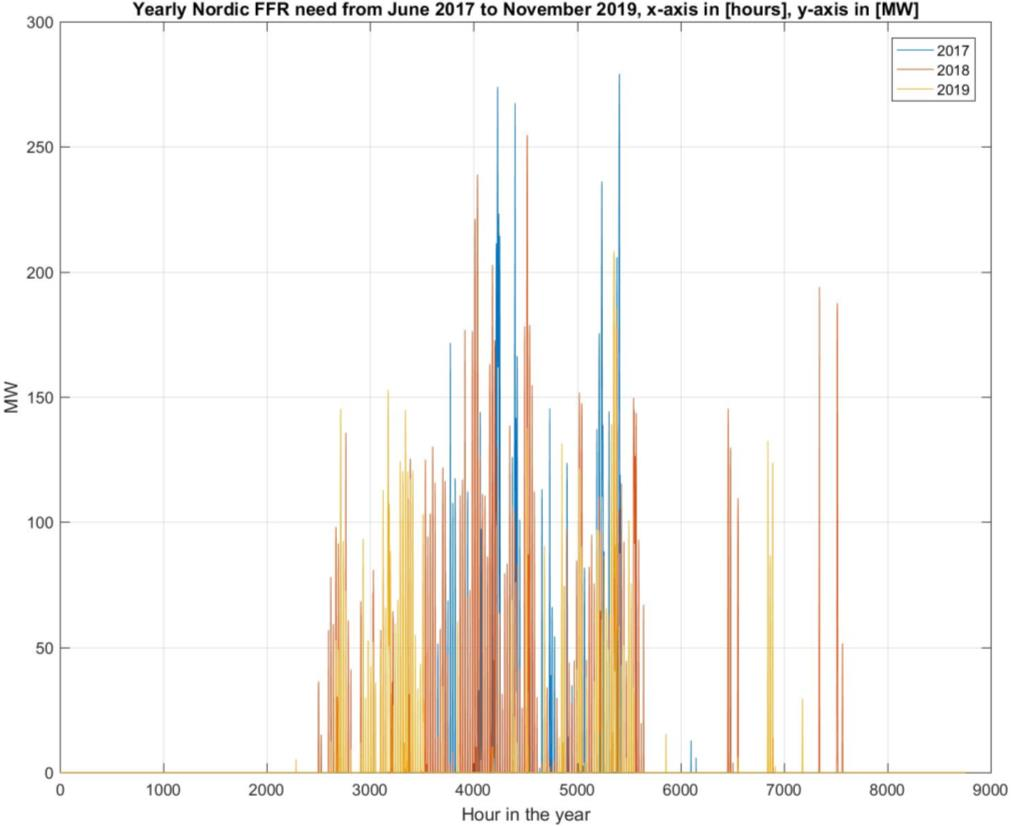
\includegraphics[scale=0.3]{Figures/FFREstimate2.jpg}
\caption{\tiny Historical need for FFR in the Nordic SA based upon estimated inertia levels from June 2017 to Nov. 2019)
}\end{figure}
\column{0.5\textwidth}
\begin{figure}
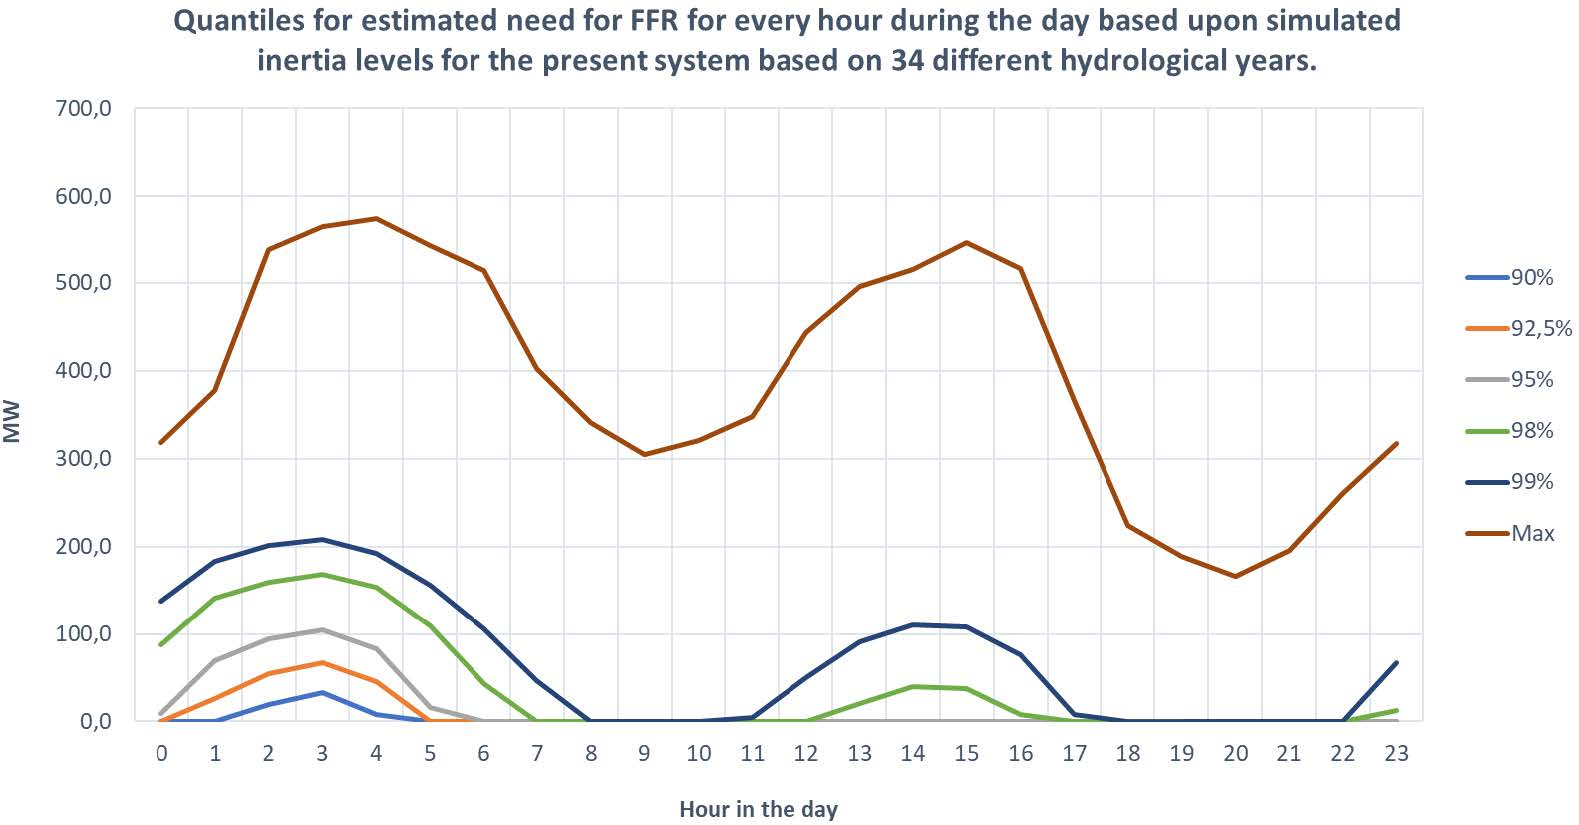
\includegraphics[scale=0.3]{Figures/FFREstimate3.jpg}
\caption{\tiny 90, 92.5, 95, 98, 99 and 100 \% quantiles for the estimated need for FFR for the Nordic SA for every hour during the day based upon simulated inertia levels for the present system based on 34 different hydrological years.
}\end{figure}
\end{columns}}
\end{frame}


%%%%%%%%%%%%%%%%%%%%%%%%%%%%%%%%%%%%%%%%%%
%%%%%%%%%%%%%%%%%%%%%%%%%%%%%%%%%%%%%%%%%%
%%%%%%%%%%%%%%%%%%%%%%%%%%%%%%%%%%%%%%%%%%
%%%%%%%%%%%%%%%%%%%%%%%%%%%%%%%%%%%%%%%%%%

\begin{frame}{Statnett Pilot for FFR, 2018}
\begin{block}{Aim to gain knowledge}
\begin{itemize}
\item about availability of such a new reserve product.
\item challenge and possibility related to technical and market aspect.
\item provide the Norwegian stakeholders with a heads-up on the future possible system needs.
\end{itemize}
\end{block}
\end{frame}
%%%%%%%%%%%%%%%%%%%%%%%%%%%%%%%%%%%%%%%%%%
%%%%%%%%%%%%%%%%%%%%%%%%%%%%%%%%%%%%%%%%%%
%%%%%%%%%%%%%%%%%%%%%%%%%%%%%%%%%%%%%%%%%%
%%%%%%%%%%%%%%%%%%%%%%%%%%%%%%%%%%%%%%%%%%
\begin{frame}{Statnett Pilot for FFR, 2018}
\begin{block}{Product requirements}
\begin{itemize}
\item Activation for a frequency triggering point of 49.6 Hz
\item Time of full activation from 49,6 Hz: 2 seconds
\item Duration: 30 seconds (i. e. FFR shall be able to be activated for a minimum of 30 seconds)
\item Resting time: 15 min
\end{itemize}
\end{block}

\begin{figure}
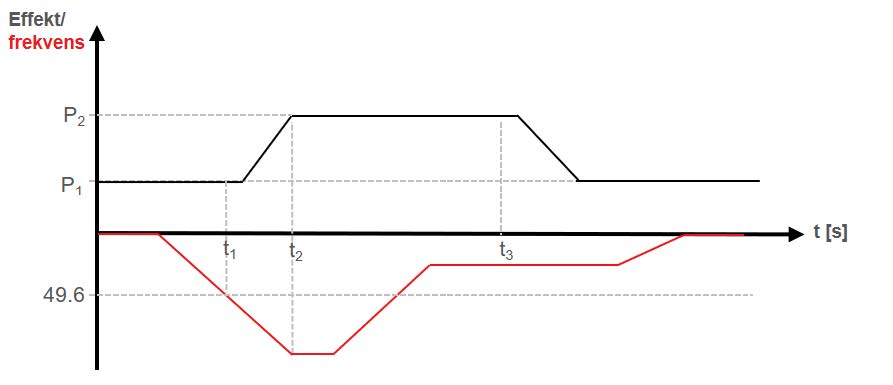
\includegraphics[scale=0.4]{Figures/ProdPilot2018.jpg}
\caption{\tiny Illustration of power response as a result of frequency change. The figure illustrates a case where netpower input to the grid is increased. [Fast Frequency Reserves 2018-pilot for raske frekvensreserver, Statnett]}

\end{figure}
\end{frame}
%%%%%%%%%%%%%%%%%%%%%%%%%%%%%%%%%%%%%%%%%%
%%%%%%%%%%%%%%%%%%%%%%%%%%%%%%%%%%%%%%%%%%
%%%%%%%%%%%%%%%%%%%%%%%%%%%%%%%%%%%%%%%%%%
%%%%%%%%%%%%%%%%%%%%%%%%%%%%%%%%%%%%%%%%%%
\begin{frame}{Statnett Pilot for FFR, 2018}
\begin{block}{Received Tenders}
\begin{itemize}
\item SFE\footnote{Song og Fjordane Energi}: Fast response form hydro power in generation mode
\item BKK: Fast load disconnection via pump power disconnection
\item Fast load reduction in a smelter (electrolysis process)
\item Fast load disconnection by an aggregated portfolio in industrial costumers.
\item Tibber: Fast load disconnection by an temporary stopping the charging in an aggregated pool of electric vehicles
\item Fortum/Basefarm: Fast switch in power supply from grid to battery power (UPS) to a data center. 
\end{itemize}
\end{block}
\end{frame}

%%%%%%%%%%%%%%%%%%%%%%%%%%%%%%%%%%%%%%%%%%
%%%%%%%%%%%%%%%%%%%%%%%%%%%%%%%%%%%%%%%%%%
%%%%%%%%%%%%%%%%%%%%%%%%%%%%%%%%%%%%%%%%%%
%%%%%%%%%%%%%%%%%%%%%%%%%%%%%%%%%%%%%%%%%%
\begin{frame}
\begin{columns}
\column{0.4\textwidth}
\begin{figure}

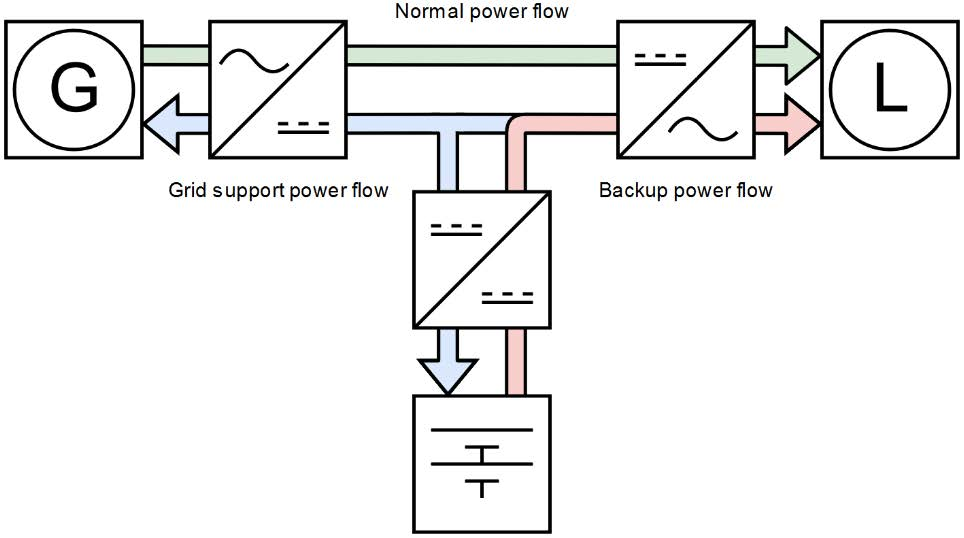
\includegraphics[scale=0.3]{Figures/fast-frequency-reserves-pilot-2018.jpg}
\caption{\tiny Power flow for UPS for normal use and for backup solution and FFR (Fortum 2018).}
\end{figure}

\column{0.6\textwidth}
\begin{figure}
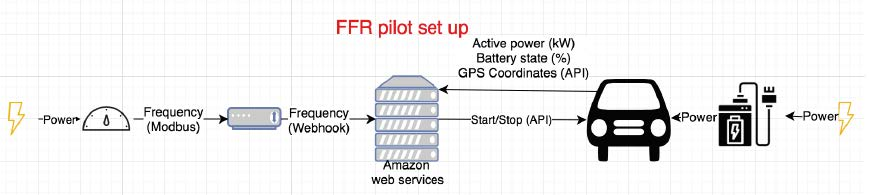
\includegraphics[scale=0.4]{Figures/fast-frequency-reserves-pilot-20181.jpg}
\caption{\tiny Delivery of FFR from electric cars (Tibber 2018)}
\end{figure}
\begin{figure}
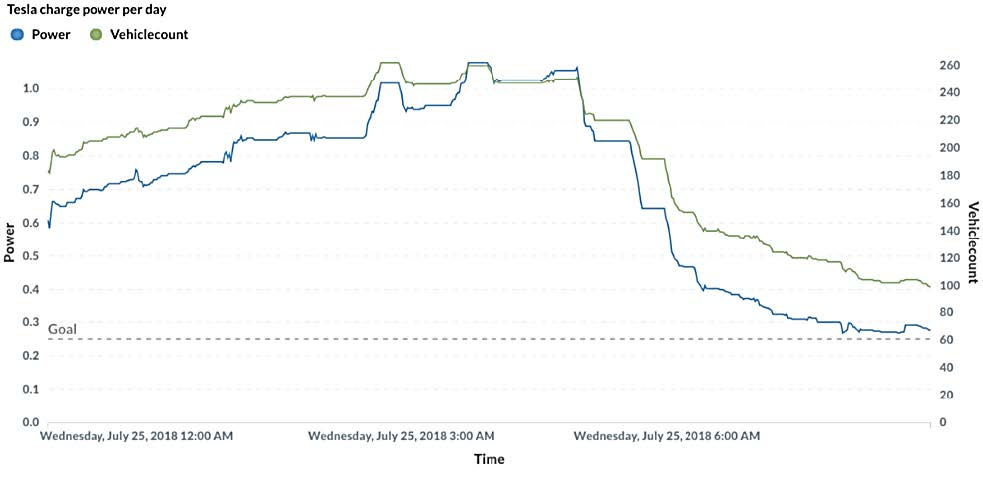
\includegraphics[scale=0.4]{Figures/fast-frequency-reserves-pilot-20182.jpg}
\caption{\tiny Example of how a portfolio of electric cars is charged through the night measured in MW (Tibber 2018).}
\end{figure}
\end{columns}
\end{frame}

%%%%%%%%%%%%%%%%%%%%%%%%%%%%%%%%%%%%%%%%%%
%%%%%%%%%%%%%%%%%%%%%%%%%%%%%%%%%%%%%%%%%%
%%%%%%%%%%%%%%%%%%%%%%%%%%%%%%%%%%%%%%%%%%
%%%%%%%%%%%%%%%%%%%%%%%%%%%%%%%%%%%%%%%%%%
\begin{frame}{Statnett Pilot for FFR, 2018}
\begin{block}{Summary of technology and fulfillment if criteria}

\end{block}
{\tiny
\begin{center}
\begin{tabular}{ l c  c c c c} 
\hline
\rowcolor{Gray} Technology & Response time &Endurance & Ramping back& Rest time  \\
\hline
\hline
Hydropower SFE& Not Ok& Ok &Ok &Ok \\
\hline
\rowcolor{Gray} Pumped-storage hydroelectricity& Ok &Ok &Not Ok& Not Ok \\
\hline
Industry, Electrolysis process & Ok& Ok& Ok& Ok\\
\hline
\rowcolor{Gray} Tibber, Aggregator, EV& Ok & Ok& Ok& Ok\\
\hline
Fortum, UPS& Ok& Ok& Ok&Ok\\
\hline
\end{tabular}
\end{center}}
\end{frame}
%%%%%%%%%%%%%%%%%%%%%%%%%%%%%%%%%%%%%%%%%%
%%%%%%%%%%%%%%%%%%%%%%%%%%%%%%%%%%%%%%%%%%
%%%%%%%%%%%%%%%%%%%%%%%%%%%%%%%%%%%%%%%%%%
%%%%%%%%%%%%%%%%%%%%%%%%%%%%%%%%%%%%%%%%%%
\begin{frame}{FFR-demo 2020}
\vskip -0.4cm
\begin{block}{}{\tiny
Statnett requested even for more faster response for FFR participants demonstration projects of 2020.}
\end{block}
\vskip -0.2cm
{\tiny
\begin{center}
\begin{tabular}{ c c  c } 
\hline
\rowcolor{Gray} Alternative& Activation level [Hz]&Maximum full activation time [s] \\
\hline
\hline
A& 49.7&1.3\\
\hline
\rowcolor{Gray} B&49.6&1.0\\
\hline
C&49.5&0.7\\
\hline
\end{tabular}
\end{center}}
\vskip -0.2cm
\begin{figure}
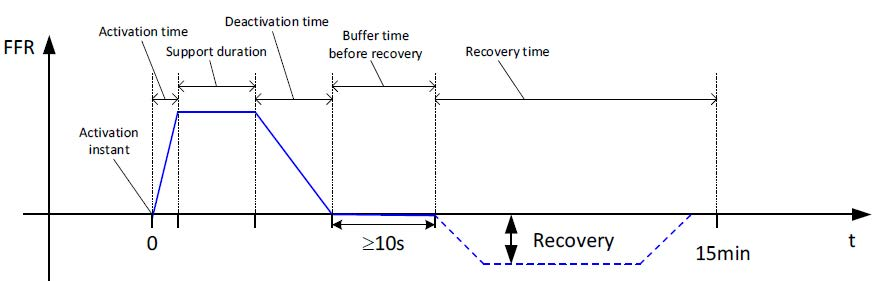
\includegraphics[scale=0.4]{Figures/FFRIGJustification Report.jpg}
\caption{\tiny Illustration of power response as a result of frequency change. The figure illustrates a case where netpower input to the grid is increased. Table and figure are taken from [FFR-demo 2020, betingelser for deltagelse i demonstrasjonsprosjekt]}
\end{figure}\vskip -0.8cm
\begin{alertblock}{} {\tiny
The Nordic product requirements define two equivalent combinations of delivery time (period of fullpower supply) and deactivation of power supply
\begin{enumerate}[I]
\item Long delivery time, at least 30 seconds
\item Short delivery time, at least 5 seconds
\end{enumerate}}
\end{alertblock}


\end{frame}
%%%%%%%%%%%%%%%%%%%%%%%%%%%%%%%%%%%%%%%%%%
%%%%%%%%%%%%%%%%%%%%%%%%%%%%%%%%%%%%%%%%%%
%%%%%%%%%%%%%%%%%%%%%%%%%%%%%%%%%%%%%%%%%%
%%%%%%%%%%%%%%%%%%%%%%%%%%%%%%%%%%%%%%%%%%
\section{Checkpoint II}
\begin{frame}{Checkpoint II}
\centering \begin{block}{}
\textbf{Summary:}
\end{block} 
\end{frame}

\begin{frame}{Summary}
\begin{block}{Highlights}
{\scriptsize
\begin{itemize}
\item<1-> Amount of inertia in the synchronous power system is proportional to the amount of rotating mass of synchronous generators and machines.
\item<2-> Massive integration of renewable energy generations, decommissioning of thermal and nuclear power plants (with synchronous generators), more and more dependence on HVDC import/export, all are parts of the road map toward expected near future.
\item<3-> TSO have an important role in shaping new emerging markets, by opening dialogue with market players and introduce flexibility in a socio-economical manner.
\item<4-> Pilot Project 2018:
\begin{enumerate}[I]
{\scriptsize
\item FFR is a cost efficient measure for handling of low inertia challenges.
\item Pilot project gave a profound understanding how FFR could be implemented and tested.
\item Pilot project gave an overview of how  flexibility could contribute to power system operational security. 
}



\end{enumerate}       
\end{itemize}
}
\end{block}
\end{frame}

\begin{frame}
\centering
Thank you for your attention!\\
		\vskip 0.8cm

\centering

\includegraphics[scale=0.2]{ntnulogo_eng.png}
\end{frame} 

\end{document}


